\chapter{Conception}


%% ------------------------------------------ %%
%%               ARCHITECTURE                 %%
%% ------------------------------------------ %%
\section{Architecture du système}\label{conception.architecture}

\subsection{Capture des images}
Cette section présente l'architecture du système de capture d'image du parking, nécessaire à ce projet. Une caméra IP sera choisie, qui sera connectée au réseau de la HEIG-VD de la manière décrite ici. La capture d'image a été pensée afin de permettre la connexion de multiples caméras.

Il faudra remarquer que les choix effectués ici non seulement influence la caméra qui sera choisie en section \ref{conception.techno.camera} \itnameref{conception.techno.camera}, mais aussi, ces choix dépendent de celle-ci. Ainsi, ces deux travaux (choix de l'architecture de capture d'image et choix de la caméra) ont été réalisés en parallèle.

\subsubsection{Architecture logique}\label{conception.architecture.capture.logique}
%\nomenclature{VM}{machine virtuelle, pour \textit{Virtual Machine} en anglais}
%\newacronym[longplural={Virtual Machines}]{VM}{VM}{Virtual Machine}

%\todo{NOMENCLATURE PAS FONCTIONNEL}
 
La caméra réseau sera connectée au réseau local de la HEIG-VD. Elle aura donc une adresse IP, qu'il sera possible d'utiliser afin de communiquer avec elle. Une machine virtuelle (abrégée \textit{VM}, pour \textit{Virtual Machine}) a été mise à disposition de ce projet. Située sur le réseau de l'école, elle permettra de récupérer ses images.

\begin{figure}[!ht]
    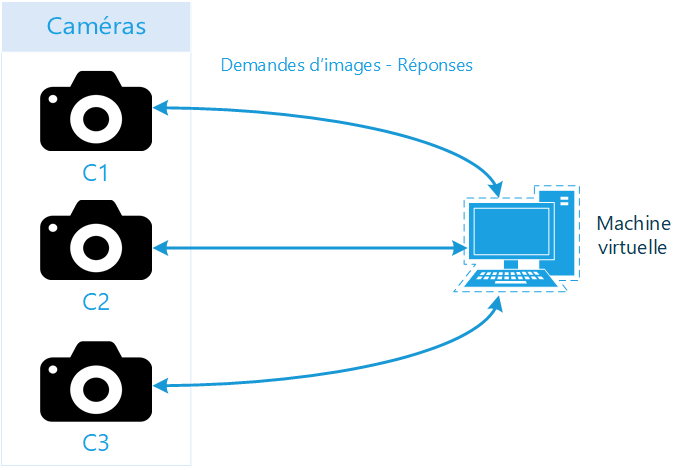
\includegraphics[width=110mm]{img/conception/logic_arch.png}
    \centering
    \caption{Capture d'images de plusieurs caméras}
    \label{fig:capture_cameras}
\end{figure}

La figure \ref{fig:capture_cameras} présente un protocole de demande-réponse sur \textit{HTTP} qui sera utilisé afin de récupérer des images à intervalles réguliers. Il est possible de la préciser ainsi:

\begin{enumerate}
    \item La \textit{VM} émet une requête demandant l'image du parking à une caméra. 
    \item La caméra répond à la \textit{VM} avec ladite image.
\end{enumerate}

Les requêtes et réponses précitées sont fortement dépendantes de la caméra choisie. Ainsi, les détails d'implémentation pourront être trouvés en section \ref{realisation.capture} \itnameref{realisation.capture}.


\subsubsection{Architecture physique}\label{conception.architecture.camera.physique}
\paragraph{Positionnement de la caméra}\label{conception.architecture.camera.physique.position}
La caméra doit pouvoir être capable de capturer des images de parking. Pour ce faire, une caméra sera installée sur le toit de la HEIG-VD. 

Il faut remarquer que l'installation de périphériques sur la terrasse n'y est pas des plus aisée. De plus, l'édification d'une salle de conférence y a débuté en date du 26 février 2018\footnote{Informations tirées d'un mail envoyé aux collaborateurs et étudiants de la HEIG-VD en date du 22 février 2018}, ne facilitant pas l'installation. Il en sera tenu compte lors du choix de la caméra. Plus d'informations concernant l'installation de celle-ci sont disponibles en section \ref{realisation.capture} \itnameref{realisation.capture}.

\paragraph{Connexion de la caméra}

Ici, deux points sont principalement étudiés: l'alimentation de la caméra, et sa connexion au réseau local de la HEIG-VD.  

\begin{figure}[H]
    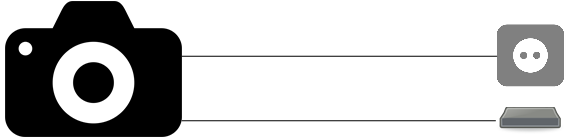
\includegraphics[width=110mm]{img/conception/cam_con_1.png}
    \label{fig:cam_connection_1}
    \centering
    \caption{Caméra alimentée et connectée au réseau par câble}
\end{figure}

La caméra pourrait être câblée au réseau électrique, ainsi qu'au réseau local. Il est nécessaire de tirer 2 câble, à 2 endroits différents: l'un au réseau électrique, et l'autre à un switch ou une prise Ethernet présente dans le bâtiment.

\begin{figure}[H]
    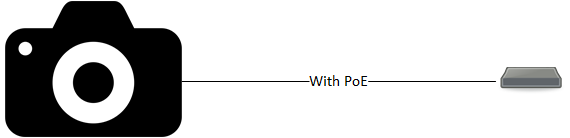
\includegraphics[width=110mm]{img/conception/cam_con_2.png}
    \label{fig:cam_connection_2}
    \centering
    \caption{Caméra câblée au réseau et alimentée par \textit{PoE}}
\end{figure}

Elle pourrait aussi être câblée uniquement au réseau local. En effet, il serait possible de profiter de la technologie \textit{Power over Ethernet} (\textit{PoE}) permettant de fournir en électricité un périphérique réseau via le câble Ethernet. Il faut cependant noter que le switch connecté à la caméra doit pouvoir fournir cette fonctionnalité.

\begin{figure}[H]
    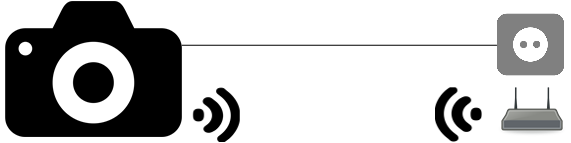
\includegraphics[width=110mm]{img/conception/cam_con_3.png}
    \label{fig:cam_connection_3}
    \centering
    \caption{Caméra alimentée par câble et connectée au réseau en Wifi}
\end{figure}

La caméra pourrait être connectée au réseau électrique par câble. La connexion au réseau local pourrait être effectuée par Wifi. Il faut cependant noter que le Wifi doit être puissant et fiable: la caméra, installée à l'extérieur du bâtiment, pourrait ne pas capter suffisamment un signal provenant de l'intérieur, ceci dû aux larges murs en bêton. 

\begin{figure}[H]
    
\includegraphics[width=110mm]{img/conception/cam_con_4.png}
    \label{fig:cam_connection_4}
    \centering
    \caption{Caméra auto-alimentée et connectée en Wifi}
\end{figure}

Une batterie, ou un panneau solaire, pourrait l'alimenter. Munie du Wifi, cette solution ne demanderait aucun câblage. On notera cependant que le prix d'un tel équipement pourrait être élevé.

\subparagraph{Solution choisie}

Comme indiqué au paragraphe \itnameref{conception.architecture.camera.physique.position}, la construction d'une salle pourrait compromettre l'installation de câble. C'est pourquoi une caméra auto-suffisante sera préférée. Ainsi:
\begin{itemize}
    \item La caméra devra pouvoir fournir une connexion puissante et fiable à un signal Wifi.
    \item Elle sera auto-alimentée. De préférence, un panneau solaire sera utilisé afin que des changements de batteries ne soient pas nécessaires.
\end{itemize}

\subsection{Distribution des informations à l'utilisateur}

\todo{Info à l'utilisateurs}

%% ------------------------------------------ %%
%%           CHOIX TECHNOLOGIQUES             %%
%% ------------------------------------------ %%

\section{Choix technologiques}

\subsection{Caméra réseau}\label{conception.techno.camera}
Une caméra réseau fournissant des images de qualités dans un prix raisonnable est nécessaire dans ce projet. Celle-ci sera utilisée principalement dans 2 buts, précisés ci-après.

\paragraph{Entrainement du modèle}
Dans un premier temps, il s'agit d'entrainer le modèle à partir des images fournies par la caméra. Pour ce faire, il doit être possible de capturer et sauvegarder des photos à intervalles réguliers. Ces images seront ensuite annotées, puis utilisées pour entrainer le modèle du réseau de neurones à convolutions. 

\paragraph{Utilisation du modèle}
Une fois le modèle définit, le but de ce projet est de l'utiliser afin de détecter le nombre de voitures présentes sur le parking. Ainsi, dans un second temps, la caméra doit pouvoir fournir des images du parking "en direct", dans le but d'obtenir un état courant du parking. Il faut noter qu'ici, la notion "en direct" désigne un intervalle de capture "relativement court", soit de l'ordre de la minute. En effet, en tant qu'utilisateur, obtenir le taux d'occupation du parking à la minute près semble suffisant. Bien entendu, un intervalle plus court entre chaque prise, ou un flux vidéo, est un plus.

Il convient donc d'effectuer l'achat d'une caméra permettant le bon déroulement de ce projet. Pour ce faire, plusieurs caméras ont été évaluées. On rencontrera donc dans les prochaines sections les contraintes et critères nécessaires à une bonne évaluation. Elles seront notées, ce qui permettra d'en retirer celle qui convient le mieux à ce projet.

Il est important de noter qu'idéalement, des tests en condition réelle des différentes caméras auraient dû être effectués. Cependant, dans le cadre de ce travail de Bachelor, le budget mis à disposition ne peut le permettre. C'est pourquoi une seule caméra sera choisie sur la base des critères définis.

\subsubsection{Contraintes}\label{conception.techno.camera.contraintes}
Comme vu en section \ref{conception.architecture.camera.physique} \itnameref{conception.architecture.camera.physique}, installer une caméra sur le toit de la HEIG-VD a pour conséquence que certaines contraintes, tant d'ordre techniques qu'organisationnelles, doivent être respectées. Celles-ci sont explicitées dans cette section.

\paragraph{Capture d'images}
La caméra devra au minimum permettre la capture d'images à intervalles réguliers d'une façon ou d'une autre. L'intervalle minimum de capture est de l'ordre de la minute, afin de pouvoir obtenir l'état courant du parking filmé. La capture de vidéos n'est pas nécessaire. On notera que si celle-ci ne fournit malheureusement que la fonctionnalité de capture vidéo, il serait tout de même possible d'en extraire des images utilisables. 

\paragraph{Usage extérieur}
La caméra doit être prévue pour un usage extérieur, avec une protection contre les intempéries (pluie, neige, froid, chaud, etc.)

\paragraph{Caméra auto-alimentée}
Comme vu en section \ref{conception.architecture.camera.physique}, la caméra doit être auto-alimentée et non câblée. Ainsi, une combinaison de batteries et de panneaux solaires semble être idéal. On peut noter que l'utilisation de batteries uniquement est envisageable dans le cadre d'un prototypage, mais ce uniquement si le remplacement de celles-ci doit être effectué à intervalles relativement éloignés, de l'ordre de la semaine.

\paragraph{Connexion réseau}
En lien avec le paragraphe précédent, la caméra doit nécessairement avoir une interface Wifi permettant de se connecter au réseau de l'école. Une connexion par Ethernet n'est pas envisageable.

\paragraph{Résolution d'image}
Dans le but d'obtenir des images de qualités suffisantes, la résolution de l'image capturée devra nécessairement être au minimum de 1280x720 pixels.

\subsubsection{Critères}
Plusieurs critères ont été définis. Chacune des caméras retenues sera notée selon ceux-ci. On les trouvera ci-après, où leur pondération sont indiqués entre crochets ([]). Une pondération élevée signifie une plus grande importance de ce critère.

\paragraph{Qualité d'image [1]}
La caméra doit avoir une bonne qualité d'image. On jugera:
\begin{itemize}
    \item La résolution de l'image. Celle-ci doit être d'au minimum 1280x720 pixels.
    \item La qualité de l'image (si possible).
\end{itemize}

\paragraph{Fonctionnalités réseaux [2]}
La caméra doit pouvoir fournir des images via le réseau et il doit être possible d'en récupérer à intervalles réguliers. Pour ce faire, on pensera à des protocoles comme les suivants: 
\begin{description}
    \item[ONVIF (Open Network Video Interface Forum)] Standard industriel ouvert permettant de contrôler, configurer et communiquer avec des caméras de sécurité IP. Permet notamment la lecture de flux vidéo en temps réel et la capture de photos \autocite{wiki:onvif}
    \item[RTSP (Real Time Streaming Protocol)] Développé par RealNetworks, Netscape et Columbia University, protocole de communication permettant de lire en temps réel un flux vidéo. \autocite{wiki:RTSP}
    \item[Requêtes HTTP] Il pourrait être possible de capturer et de récupérer à la demande une photo à l'aide de requêtes HTTP.
    \item[Flux sur HTTP] Permet la lecture de flux vidéo sur HTTP en s'appuyant sur des formats tel que MPEG-4.
    \item[Interface Web HTTP] Permet la configuration de la caméra IP via un serveur Web qu'elle expose. 
    \item[FTP] La caméra peut exposer un serveur FTP contenant les photos capturées. Elle pourrait aussi téléverser des photos capturées sur un serveur FTP distant.

Il est important de préciser qu'on évaluera avant toute sur la facilité d'utilisation des différents protocoles.
\end{description}

\paragraph{Fonctionnement auto-alimenté [4]}
La caméra doit être auto-alimentée et non câblée. Comme critères, on pensera donc à:
\begin{itemize}
    \item La durée de vie de la caméra en fonctionnement auto-alimenté. Idéalement, la caméra ne devrait nécessiter aucune intervention humaine.
    \item La portée du Wifi. La puissance du signal doit être assez forte afin de pouvoir capter les bornes Wifi de l'école situées à l'intérieur depuis le toit de la HEIG-VD. Il est important de noter que ce critère peut être difficilement évalué avant l'achat de la caméra.
\end{itemize}

\paragraph{Capture de photo [2]}
La caméra doit être capable de fournir un moyen pour capturer des photos à intervalles réguliers, de l'ordre de la minute. Pour ce faire, la caméra peut fournir un système de capture de photos automatique, ce qui est un plus. On évaluera donc les moyens fournis par la caméra permettant ces captures.

\paragraph{Angle de vue [2]}
L'angle de vue de la caméra doit être suffisamment grand afin d'obtenir une image du parking dans son ensemble. Il peut être suffisant à partir de 40°, de par la hauteur à laquelle elle sera placée. Cependant, un angle de 90° semble plus satisfaisant. Ces angles ont été définis à l'aide des informations fournies par \url{videosurveillance-boutique.fr} \autocite{cam:securite_info}.

\paragraph{Vision de nuit [1]}
Idéalement, la caméra devrait pouvoir fournir une vision de nuit afin de pouvoir capturer des images de parking par toute heure. On pensera notamment aux matinées et aux soirées d'hiver, où les véhicules arrivent et partent alors que la luminosité est encore très faible. Cependant, dans le cadre de ce TB, cette fonctionnalité n'est pas strictement nécessaire.

\paragraph{Facilité d'installation [1]}
La facilité d'installation de la caméra sera prise en compte. On pensera aux dimensions de celle-ci, à son poids, au nombre de ses composants (par exemple, est-il nécessaire d'installer une batterie en plus de la caméra, ou est-elle incorporée à celle-ci?), ou encore aux accessoires fournis pour son installation. 

\paragraph{Prix [4]} Bien évidemment, le prix doit entrer en ligne de compte. 100.- CHF sera indiqué comme prix maximum afin d'obtenir la meilleure note. A partir de 500.- CHF, on évaluera ce prix comme étant mauvais.

\subsubsection{Caméras disponibles et évaluation}
Bien que la surveillance n'est pas un but de ce projet, les caméras de sécurités semblent être les plus adaptées. En effet, elles fournissent généralement des fonctionnalités de capture de photos, de connexion réseau, de vision de nuit, possèdent un angle de vue suffisant et sont souvent résistantes à un environnement extérieur. De plus, elles sont spécialement conçues pour un usage qui s'apparente à celui de ce TB, et sont donc adaptées à la prise d'images de parking.

L'achat distinct d'une caméra, de panneaux solaires et de batteries est envisageable. Néanmoins, dans un premier temps, seuls des kits complets (caméra, batteries, panneaux solaires) ont été analysés. En effet, l'installation et le choix des différents composants nécessaires à un système solaire complet semble difficile lorsqu'on est pas du domaine, et des problèmes d'interopérabilité pourraient survenir. Ceci reste cependant une solution viable si aucun kit ne correspond aux contraintes définies.

De part les contraintes très spécifiques précisées jusqu'ici, le nombre de caméras les satisfaisant toutes est faible. On trouvera ci-après les kits complets solaires auto-suffisants qui ont été évalués. Il faut aussi noter que seules les caméras les plus appropriées sont indiquées ici.

\paragraph{\textbf{Electrosun} -- Caméra-surveillance-solaire}
\textit{Electrosun} est une entreprise de domotique solaire française. Entre autres, un kit solaire de caméra complet est mis en vente. \autocite{cam:electrosun_site}

\begin{figure}[ht]
    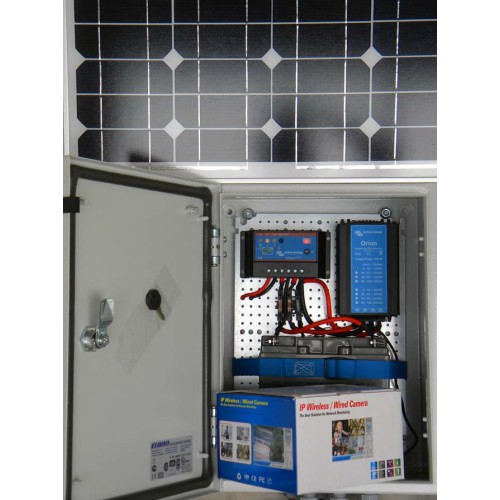
\includegraphics[width=50mm]{img/conception/electrosun_cam.jpg}
    \centering
    \captionsource{\textbf{Electrosun} Caméra de surveillance solaire}{cam:electrosun_site}
\end{figure}

Bien qu'elle satisfasse la plupart des contraintes, elle n'a pas été retenue pour l'évaluation. En effet, la résolution des images capturées n'est que de 640x480 pixels, ce qui n'est pas suffisant.

\paragraph{\textbf{Reolink} -- Argus 2}
L'entreprise \textit{Reolink} développe des caméras 100\% sans fil, avec batteries rechargeables et panneaux solaires. Elle est auto-suffisante.\autocite{cam:argus2}

\begin{figure}[ht]
    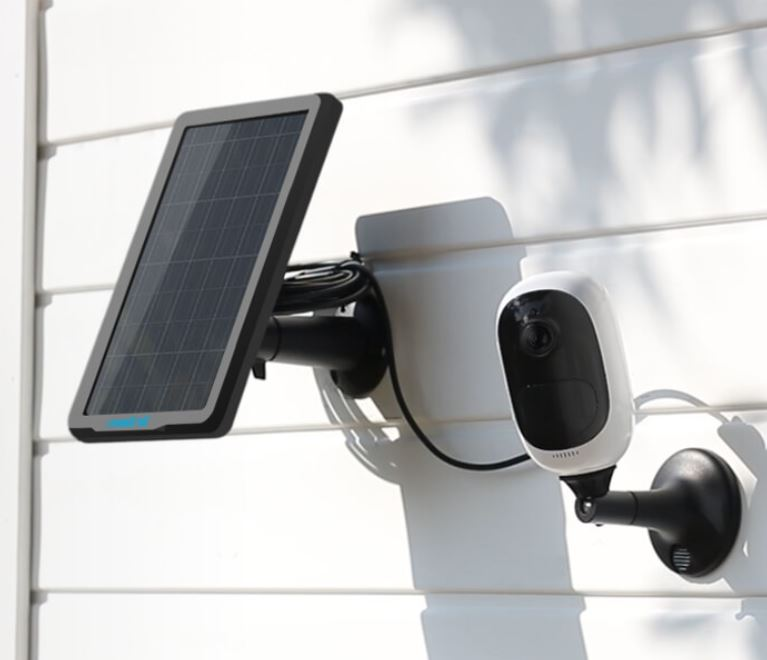
\includegraphics[width=50mm]{img/conception/argus2_cam.jpg}
    \centering
    \captionsource{\textbf{Reolink} Argus 2}{cam:argus2}
\end{figure}

Elle permet de capturer des photos FullHD (1920x1080 pixels), possède une fonction de vision de nuit ou encore, l'utilisation en extérieur est possible. Cependant, cette caméra n'a elle non plus pas pu être prise en considération. En effet, elle a été pensée pour un usage privé, et bien que la caméra puisse être connectée à un réseau Wifi, l'accès à celle-ci n'est possible qu'à l'aide d'une application smartphone (tel que décrit dans les spécifications disponibles sur le site officiel \url{https://reolink.com/product/argus-2}\autocite{cam:argus2}). Récupérer des photographies à intervalles réguliers semble donc difficilement réalisable.

\paragraph{\textbf{Wanscam} -- HW0029-3}

\textit{Wanscam} est une entreprise chinoise spécialisées dans la production de caméra réseau. Plusieurs versions de son modèle \textit{HW0029} sont disponibles. Ici est présenté le modèle \textit{HW0029-3}. \autocite{cam:wan3}

\begin{figure}[ht]
    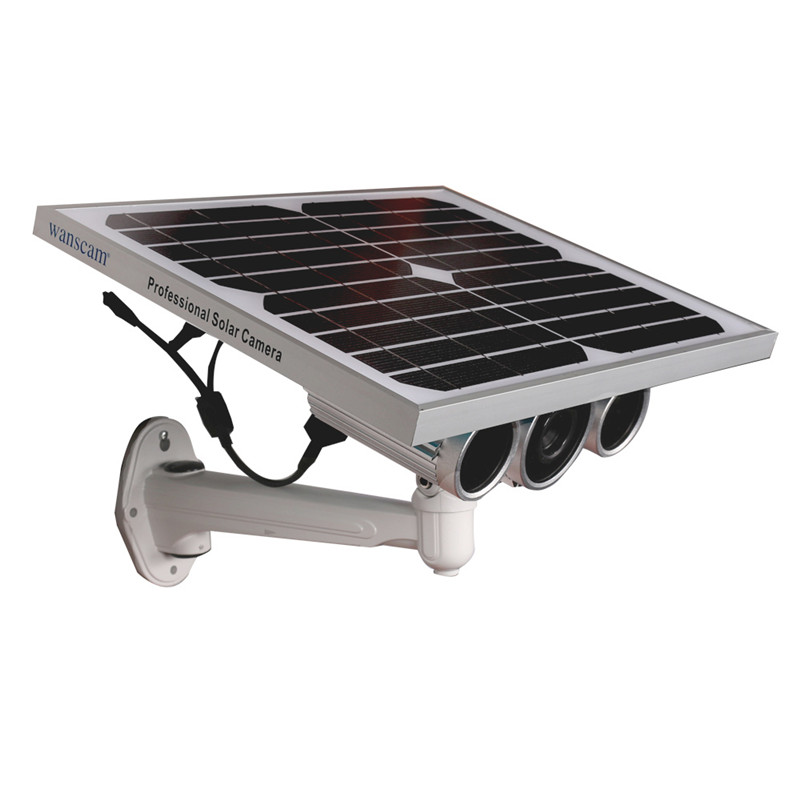
\includegraphics[width=50mm]{img/conception/wan3_cam.jpg}
    \centering
    \captionsource{\textbf{Wanscam} HW0029-3}{cam:wan3}
\end{figure}

Cette caméra satisfait toutes les contraintes définies en section \ref{conception.techno.camera.contraintes}. On trouvera en table \ref{tab:HW0029-3} ses principales caractéristiques.\footnote{Tirées des spécifications officielles \autocite{cam:wan3} et d'un test indépendant \autocite{cam:wan3-test}.}

\begin{table}[H]
    \centering
    \caption{Caractéristiques de la caméra \textbf{Wanscam} \textit{HW0029-3}}
    \label{tab:HW0029-3}
    \begin{tabular}{@{}ll@{}}
    \toprule
    Caractéristique        & Valeurs                                                                                                                                                                                                                                                                                     \\ \midrule
    Image                  & 1280 x 720, 25fps, compression H.264                                                                                                                                                                                                                                                        \\ [0.8ex]
    Angle de vue           & 40°                                                                                                                                                                                                                                                                                         \\ [0.8ex]
    Vision nocturne         & Visibilité jusqu'à 15 mètres                                                                                                                                                                                                                                                                \\ [0.8ex]
    Réseau                 & RJ45, Wifi 802.11 b/g/n                                                                                                                                                                                                                                                                     \\ [0.8ex]
    Auto-alimentation      & \begin{tabular}[c]{@{}l@{}}2 batteries de 12A et panneau solaire. \\ Sans soleil: 48h d'utilisation. \\ Faible température (\textless 26°) des rayons de soleil: 7 jours d'utilisations. \\ Grande température (\textgreater 33°) des rayons de soleil: fonctionnement continu\end{tabular} \\ [0.8ex]
    Stockage               & Carte MicroSD de 16Gb incluse, support jusqu'à 128Gb                                                                                                                                                                                                                                        \\ [0.8ex]
    Détection de mouvement & Oui                                                                                                                                                                                                                                                                                         \\ [0.8ex]
    Accès aux images       & Flux HTTP, ONVIF, RTSP, requêtes HTTP                                                                                                                                                                                                                                                       \\ [0.8ex]
    Dimensions et poids    & 370x290x110 mm, 2.7 kg                                                                                                                                                                                                                                                                      \\ \bottomrule
    \end{tabular}
\end{table}

On notera que le panneau solaire est fixé sur la caméra. Ainsi, dans le but de garder une exposition au soleil suffisante, l'angle de la caméra ne doit pas être trop élevé. Il y a donc certaines contraintes à l'installation de celle-ci.

Concernant la capture d'image, la caméra fournit des \textit{endpoints HTTP} (dont une liste peut être trouvée sur le site \url{tutoriels.domotique-store.fr}\autocite{cam:wan3-url}) permettant de récupérer l'image actuelle. Il est donc facile d'imaginer un simple agent qui, à intervalle régulier, demandera à la caméra une image, et la sauvegardera en local.

Les caméras \textbf{Wanscam} ne sont pas des plus faciles à trouver dans le commerce. Elles sont principalement disponibles sur \url{aliexpress.com}. Le modèle \textit{HW0029-3} peut être trouvé à partir de 170CHF (en date du 09.03.2018, \url{aliexpress.com}).

La grille d'évaluation \ref{cam:wan3_eval} a pu être remplie à l'aide de ces spécifications.

\begin{table}[H]
    \centering
    \caption{Evaluation de la caméra \textbf{Wanscam} \textit{HW0029-3}}
    \label{cam:wan3_eval}
    \begin{tabular}{@{}llp{8cm}@{}}
        \toprule
        Critère                              & Note (de 1 à 5) & Remarques                                                                                                                                                                   \\ \midrule
        Qualité d'image              & 3 [1]               & La qualité d'image semble suffisante selon les tests effectués par \url{lesbonstuyauxgeeks.fr}\autocite{cam:wan3-test}. La résolution est de 1280x720 pixels, ce qui est suffisant. \\ [0.8ex]
        Fonctionnalités réseaux      & 5 [2]              & La caméra offre notamment un endpoint HTTP sur lequel récupérer les images.                                                                                                \\ [0.8ex]
        Fonctionnement auto-alimenté & 4 [4]              & La caméra est totalement auto-suffisante s'il y a assez de soleil. On notera cependant le panneau solaire fixe qui peut nuire à l'exposition du soleil. Elle supporte le Wifi 802.11n: à première vue, le signal semble suffisant.                   \\ [0.8ex]
        Capture de photo             & 5 [2]              & Il est facile de récupérer des images sur cette caméra. Elle offre en plus un système de capture de photos à intervalles réguliers automatique. Elle offre aussi la possibilité de récupérer un flux vidéo.                            \\ [0.8ex]
        Angle de vue                 & 1 [2]              & Un angle de vue de 40° semble tout juste suffisant.                                                                                                                        \\ [0.8ex]
        Vision de nuit               & 2 [1]               & Elle fournit une vision nocturne à 15m. Il est cependant possible d'ajouter des LED infrarouges supplémentaires afin d'obtenir une meilleure vision de nuit\autocite{cam:wan3-url}. \\ [0.8ex]
        Facilité d'installation      & 3 [1]              & La caméra mesure jusqu'à 37 cm, ce qui nuit à sa facilité d'installation. De plus, le panneau solaire est fixe, ce qui contraint la position et l'angle de la caméra.      \\ [0.8ex]
        Prix                         & 4 [4]              & A partir d'environ 170.- CHF \\ \midrule
        && \textbf{Note finale: 3.6/5} \\ \bottomrule
    \end{tabular}
\end{table}

\paragraph{\textbf{Wanscam} -- HW0029-5}
Le modèle \textit{HW0029-5} de \textbf{Wanscam} est la nouvelle version du modèle \textit{HW0029-3} décrit précédemment. Elle possède la plupart des mêmes caractéristiques, mais propose une meilleure résolution (1920x1080), des batteries à plus grande capacité, un meilleur champ de vision, ou encore, une vision de nuit accrue jusqu'à 100m. Son prix est cependant plus élevé que la caméra \textit{HW0029-3}. Les caractéristiques indiquées dans ce rapport proviennent du site officiel \url{wanscam.com}\autocite{cam:wan5}.

\begin{figure}[ht]
    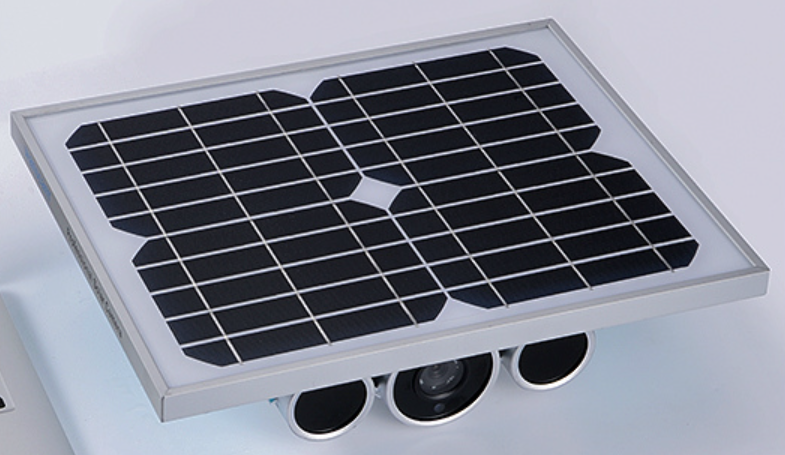
\includegraphics[width=50mm]{img/conception/wan5_cam.png}
    \centering
    \captionsource{\textbf{Wanscam} HW0029-5}{cam:wan5}
\end{figure}

\begin{table}[H]
    \centering
    \caption{Caractéristiques de la caméra \textbf{Wanscam} \textit{HW0029-5}}
    \label{tab:HW0029-5}
    \begin{tabular}{@{}ll@{}}
    \toprule
    Caractéristique        & Valeurs                                                                                                                                                                                                                                                                                     \\ \midrule
    Image                  & 1920 x 1080, 25-30fps, compression H.264                                                                                                                                                                                                                                                        \\ [0.8ex]
    Angle de vue           & 80°                                                                                                                                                                                                                                                                                         \\ [0.8ex]
    Vision nocturne         & Visibilité jusqu'à 100 mètres                                                                                                                                                                                                                                                                \\ [0.8ex]
    Réseau                 & RJ45 100Mbps, Wifi 802.11 b/g/n                                                                                                                                                                                                                                                                     \\ [0.8ex]
    Auto-alimentation      & \begin{tabular}[c]{@{}l@{}}2 batteries de 12A et panneau solaire. \\ Sans soleil: 54h d'utilisation. \end{tabular} \\
    Stockage               & Carte MicroSD de 16Gb incluse, support jusqu'à 128Gb                                                                                                                                                                                                                                        \\ [0.8ex]
    Détection de mouvement & Oui                                                                                                                                                                                                                                                                                         \\ [0.8ex]
    Accès aux images       & Flux HTTP, ONVIF, RTSP, requêtes HTTP                                                                                                                                                                                                                                                       \\ [0.8ex]
    Dimensions et poids    & 370x286x960 mm, 4.3 kg                                                                                                                                                                                                                                                                      \\ \bottomrule
    \end{tabular}
\end{table}

Il faudra noter que cette caméra est plus lourde, bien que plus petite, que le précédent modèle. 

De ces caractéristiques, il a été possible d'évaluer cette caméra dans la grille d'évaluation \ref{cam:wan5_eval} 

\begin{table}[H]
    \centering
    \caption{Evaluation de la caméra \textbf{Wanscam} \textit{HW0029-5}}
    \label{cam:wan5_eval}
    \begin{tabular}{@{}llp{8cm}@{}}
        \toprule
        Critère                      & Note (de 1 à 5) & Remarques                                           \\ \midrule
        Qualité d'image              & 4 {[}1{]}       & La qualité de l'image est meilleure que le modèle précédent, avec une résolution de 1920x1080 pixel.                                                              \\ [0.8ex]
        Fonctionnalités réseaux      & 5 {[}2{]}       & La caméra offre notamment un endpoint HTTP sur lequel récupérer les images.                                                                                       \\ [0.8ex]
        Fonctionnement auto-alimenté & 4 {[}4{]}       & De la même manière que le modèle précédent, la caméra est totalement auto-suffisante s'il y a assez de soleil. Sans soleil, elle est auto-suffisante jusqu'à 54h. Elle supporte la norme Wifi 802.11n \\ [0.8ex]
        Capture de photo             & 5 {[}2{]}       & Il est facile de récupérer des images sur cette caméra. De plus, elle offre un système de capture de photos à intervalles réguliers automatiques. Elle offre aussi la possibilité de récupérer un flux vidéo.                  \\ [0.8ex]
        Angle de vue                 & 4 {[}2{]}       & Un angle de vue de 80° semble être approprié pour ce projet. Un angle supérieur n'aurait pas été superflu.                                                        \\ [0.8ex]
        Vision de nuit               & 5 {[}1{]}       & Elle fournit une vision nocturne à 100m.                                                                                                                          \\ [0.8ex]
        Facilité d'installation      & 3 {[}1{]}       & Tout comme le modèle HW0029-3, la caméra n'est pas des plus petites, mesurant jusqu'à 37 cm. Le panneau solaire est fixé à la caméra.                             \\ [0.8ex]
        Prix                         & 3 {[}4{]}       & A partir d'environ 230.- CHF   \\ \midrule
        && \textbf{Note finale: 4.0/5} \\ \bottomrule
    \end{tabular}
\end{table}

\subparagraph{Remarque} Le modèle \textbf{Wanscam} \textit{HW0029-4} (ainsi que sa version améliorée \textit{HW0029-6}) n'a pas été pris en compte. En effet, il fourni en plus un système de puce 4G afin de pouvoir connecter la caméra à un réseau mobile. En conséquence, le prix est trop élevé, dépassant les 400.- CHF.

\paragraph{\textbf{Visortech} -- Caméra Solaire IP}
Cette caméra satisfait toutes les contraintes définies dans la section \ref{conception.techno.camera.contraintes} \itnameref{conception.techno.camera.contraintes}. Ses caractéristiques principales sont décrites à la table \ref{tab:visortech_spec}. Il a été possible de remarquer que la caméra décrite ici est disponible sous différents noms, comme \textit{IdealSmartCam}.

\begin{figure}[ht]
    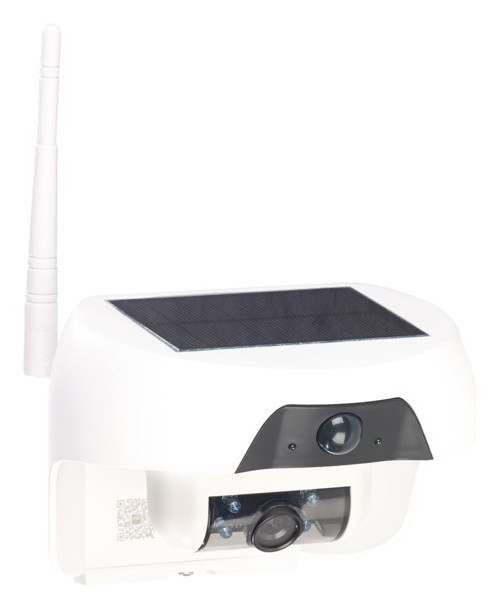
\includegraphics[width=50mm]{img/conception/visortech_cam.jpg}
    \centering
    \captionsource{Caméra Visortech}{cam:visortech}
\end{figure}

On regrettera le peu d'informations disponibles concernant les spécifications de cette caméra. Par exemple, il est difficile de connaitre les méthodes disponibles afin de pouvoir récupérer des images depuis le réseau local, tant et si bien que cela soit possible. On notera que le vendeur a été contacté, sans réponse de sa part.

\begin{table}[H]
    \centering
    \caption{Caractéristiques de la caméra \textit{Visortech}}
    \label{tab:visortech_spec}
    \begin{tabular}{@{}lp{10cm}@{}}
    \toprule
    Caractéristique        & Valeurs                                                          \\ \midrule
    Image                  & 1280 x 720, compression H.264. Prise de vue en continu possible. \\ [0.8ex]
    Angle de vue           & 90°                                                              \\ [0.8ex]
    Vision nocturne         & Visibilité jusqu'à 5 mètres                                      \\ [0.8ex]
    Réseau                 & Wifi 802.11 b/g/n                                                \\ [0.8ex]
    Auto-alimentation      & Panneau solaire intégré de 0.8 Watt, jusqu'à 5 jours sans soleil. Auto-suffisante.     \\ [0.8ex]
    Détection de mouvement & Oui                                                              \\ [0.8ex]
    Dimensions et poids    & 161x155x108 mm, 0.8 kg                                            \\  [0.8ex]\bottomrule
    \end{tabular}
\end{table}

Malgré le manque d'information, cette caméra a tout de même été évaluée. Il sera de ce fait possible de savoir si elle peut être un choix viable, ou non. La grille d'évaluation correspondante peut être trouvée en table \ref{tab:visortech_eval}

\begin{table}[H]
    \centering
    \caption{Evaluation de la caméra \textit{Visortech}}
    \label{tab:visortech_eval}
    \begin{tabular}{@{}llp{8cm}@{}}
        \toprule
        Critère                      & Note (de 1 à 5) & Remarques                          \\ \midrule
        Qualité d'image              & 3 {[}1{]}       & Sa résolution est de 1280x720 pixel.                                                                                                  \\ [0.8ex]
        Fonctionnalités réseaux      & 2 {[}2{]}       & Accès via smartphone possible, peu d'informations concernant les protocoles réseaux disponibles.                                      \\ [0.8ex]
        Fonctionnement auto-alimenté & 3 {[}4{]}       & Devrait être auto-suffisante. Cependant, informations peu claires si prises d'images en continu. Accepte la norme Wifi 802.11n. \\ [0.8ex]
        Capture de photo             & 3 {[}2{]}       & Permet l'accès au flux vidéo en direct. Peu d'informations sur les protocoles disponibles.                                            \\ [0.8ex]
        Angle de vue                 & 5 {[}2{]}       & Angle de vue de 90°. Meilleur champ de vision parmi les caméras évaluées.                                                              \\ [0.8ex]
        Vision de nuit               & 2 {[}1{]}       & Elle fournit une vision nocturne à 5m.                                                                                                \\ [0.8ex]
        Facilité d'installation      & 3 {[}1{]}       & La caméra est relativement petite, et ne pèse que 850g. On notera l'absence de pied: une fixation à un mur semble nécessaire.         \\ [0.8ex]
        Prix                         & 3 {[}4{]}       & A partir d'environ 220.- CHF                                                                                                          \\ [0.8ex]
                                    &                 & \textbf{Note finale: 3.1/5} \\ \bottomrule
    \end{tabular}
\end{table}

\subsubsection{Choix final}

La caméra \textit{Visortech} arrive dernière du classement, avec une note de 3.1. Ceci est avant tout du au manque d'informations sur les protocoles utilisables afin de récupérer via le réseau des images. Elle n'a donc pas été retenue.

\begin{table}[!ht]
    \centering
    \caption{Caméras - Synthèse des résultats}
    \label{cam:synthese}
    \begin{tabular}{@{}lll@{}}
    \toprule
      & Caméra           & Note \\ \midrule
    \textbf{1} & Wanscam HW0029-5 & 4.0  \\
    \textbf{2} & Wanscam HW0029-3 & 3.6  \\
    \textbf{3} & Visortech        & 3.1  \\ \bottomrule
    \end{tabular}
\end{table}

Les deux versions de la caméra \textit{HW0029} de \textbf{Wanscam} montrent des résultats proches. Elles sont avant tout distinguables par leur qualité d'image, leur vision de nuit, leur durée de fonctionnement sur batterie et leur angle de vue, où toutes ces caractéristiques sont améliorées sur le nouveau modèle (\textit{HW0029-5}). Ainsi, seul le rapport qualité/prix peut faire pencher la balance d'un côté ou d'un autre. Avec un peu de recherche, la version \textit{HW0029-5} a été trouvée à 187.50€ sur \url{aliexpress.com}\autocite{cam:wan5-buy} (frais de livraison inclus), soit 225.- CHF (1.17CHF/€ en date du 13 mars 2018\autocite{util:cours}, arrondi au dixième supérieur, soit 1.20 CHF/€). 

Au prix indiqué plus haut, et vis-à-vis du classement présenté en table \ref{cam:synthese}, la caméra \textbf{Wanscam} \textit{HW0029-5} a été choisie pour la capture d'image que demande ce projet.

\subsection{Langage de développement}
Afin de choisir le langage de programmation qui sera majoritairement utilisé dans ce projet, il est premièrement nécessaire de définir quel en sera son utilisation. On résumera donc ses objectifs principaux ainsi:
\begin{itemize}
    \item Le langage sera utilisé afin de capturer des images sur HTTP.
    \item Le langage sera fortement utilisé pour du traitement d'image.
    \item Le langage sera fortement utilisé pour du \textit{Machine Learning}, plus spécifiquement des réseaux de neurones à convolutions.
\end{itemize}

De ce fait, se tourner vers un langage s'approchant du \textit{script} (qu'on pourra par exemple opposer au langage \textit{Java}) semble avoir plusieurs avantages:
\begin{itemize}
    \item Le langage sera beaucoup utilisé afin de traiter des informations. Ces traitements seront relativement courts, mais multiples. Un langage de script semble suffisant.
    \item Les langages de scripts sont légers, aisément maintenables et évolutifs. Il est cependant important de noter qu'ils le sont seulement si les programmes développés restes courts et bien construits. 
    \item Les scripts ressemblent souvent à de la programmation procédurale, ce qui peut en faciliter son écriture. Puisqu'avant tout, des traitements seront effectués, un style de programmation procédurale semble idéal.
\end{itemize}

Dans le cadre de ce TB, du \textit{Machine Learning} sera effectué. Il convient donc aussi de s'informer sur les langages de développement les plus populaires utilisés dans ce contexte. On en tirera une liste, non-exhaustive. Il faut noter que cette liste a été définie par ce qui a pu être vu par l'expérience, et non par un réel classement:
\begin{description}
    \item[R] Environnement gratuit de statistiques et graphiques.\autocite{lang:R}
    \item[MATLAB] Développé par \textit{MathWorks}, combine un environnement \textit{desktop} pour de l'analyse et un langage de programmation spécialisés.\autocite{lang:matlab}
    \item[Python] Langage de programmation permettant un développement rapide et efficace. \autocite{lang:python}
\end{description}

Le choix du langage dépend aussi fortement des librairies qui sont disponibles et utilisées. Dans le cadre du \textit{Machine Learning} et du traitement d'images, elles sont très souvent disponibles en \textit{Python}.

\paragraph{Choix du langage}
De part ce qui a été précisé précédemment, \textit{Python} semble être le langage idéal. Il est possible de noter qu'il permet aussi une certaine conception orientée objet.

\paragraph{Limitation}
Une des principales limitations de ce langage et qu'il est interprété. Ainsi, les performances peuvent être plus faibles qu'un langage compilé\footnote{ On notera cependant qu'il est possible, si on le souhaite, de compiler du \textit{Python}. Là n'est cependant pas son but premier}. Cependant, et comme on le verra plus tard, les librairies fournies sont souvent des \textit{wrappers} interfaçant du code compilé. Ainsi, les traitements lourds sont souvent efficaces, où \textit{Python} peut ne servir qu'à connecter des composants et définir des configurations. 

\subsection{Traitement d'images}
Dans ce projet, une des premières étapes consiste à traiter les images provenant de la caméra afin qu'elles puissent être utilisées convenablement dans l'algorithme de \textit{Machine Learning}. On trouvera ci-après les différents traitements qui doivent pouvoir être réalisés:
\begin{description}
    \item[\textit{Downsampling}] L'image reçue de la caméra sera sous-échantillonnée.
    \item[\textit{Edge detection}] Les bords pouvant être détectés dans l'image devront pouvoir être mis en valeur. 
\end{description}

\subsubsection{Librairies disponibles}
Plusieurs librairies \textit{Python} sont disponibles. Ici en sont décrites deux.

\paragraph{OpenCV}
OpenCV\autocite{lib:opencv} (\textit{Open Source Computer Vision Library}) est une librairie Open Source permettant le traitement d'image. Elle peut être utilisée en C++, Java, et Python. Elle est écrite en C/C++ est et optimisée pour une utilisation sur un CPU multi-core. Elle permet notamment de sous-échantillonner une image et de détecter des bords, mais possède aussi beaucoup de fonctionnalités liées au \textit{Machine Learning}.

\paragraph{Scikit-image}
Scikit-image\autocite{lib:skimage}, abrégé \textit{skimage}, est une collection gratuite et Open Source d'algorithmes pour le traitement d'images en python. Elle permet aisément de sous-échantillonner des images, ainsi que de détecter des bords à l'aide de filtres prédéfinis (convolutions).

\subsubsection{Comparaison}
Les deux librairies pré-citées sont ressemblantes sur bien des points. Une image, dans les deux cas, est représentée sous la forme d'un tableau \textit{numpy}\footnote{Numpy est une librairie scientifique permettant d'utiliser en \textit{Python} des tableaux multidimensionnels de manière efficaces.\autocite{lib:numpy}} à 3 dimensions. Les syntaxes des deux librairies sont aussi extrêmement proches où, parfois même, les noms de méthodes et arguments présents se trouvent être strictement les mêmes.

On pourra cependant les différencier par deux points principaux, en relation avec ce projet:
\begin{itemize}
    \item La librairie \textit{skimage} est plus facile d'accès. Ces méthodes sont mieux définies et le traitement d'une image est plus aisé qu'avec \textit{OpenCV}. Elle offre, en plus, des fonctionnalités d'aide au développement pour le traitement d'images tri-signaux (valeurs \textit{RGB}) et leurs conversions (par exemple, en valeurs \textit{HSV} telles que décrites en section \ref{techno.traitement.repr.coul} \itnameref{techno.traitement.repr.coul})
    \item La librairie \textit{OpenCV} est plus complète. Elle possède en plus des fonctionnalités liées au \textit{Machine Learning}, comme de la détection d'objet dans une image.
\end{itemize}

\subsubsection{Choix final}
Il a donc été choisi d'utiliser au possible la librairie \textit{scikit-image}, qui est plus facile d'accès. 

Néanmoins, il est important de noter que le fait qu'une image soit représentée de la même manière dans les deux librairies permet une certaine interopérabilité entre celles-ci. \textit{Skimage} souffre de certaines limitations lorsqu'on la compare à \textit{OpenCV}, mais il est facile de les contourner: lorsque c'est nécessaire, \textit{OpenCV} pourra être utilisé en parallèle.

\subsection{Réseau de neurones}
\todo{Keras, etc.}
\subsubsection{Librairies disponibles}
\subsubsection{Comparaison}
\subsubsection{Choix final}

\section{Traitement des images}\label{conception.traitement}
Cette section présente le traitement des images qui est effectué avant qu'elles soient utilisées dans le réseau de neurones. 

\paragraph{Anonymisation}
Dans le cadre de ce TB, un point essentiel est l'anonymisation des données. En effet, la sphère privée des utilisateurs du parking du site de Cheseaux se doit d'être respectée. Un effort tout particulier sera donc pris afin d'anonymiser au mieux ces images. Notamment, les images capturées de la caméra sont traitées dès leurs arrivées, et ce même avant leurs enregistrement sur disque persistant. 

Aussi, dans ce rapport, les images de parking présentées proviennent du dataset \textit{PKLot}\footnote{\textit{PKLot} (disponible à l'adresse \url{https://web.inf.ufpr.br/vri/databases/parking-lot-database/}) est un grand dataset de plus de 12'000 images provenant de 3 parking, libre à l'utilisation.\autocite{paper:pklot}}. De ce fait, aucune image du parking de la HEIG-VD où des personnes et des modèles de voitures pourraient être distingués n'y sera présent. Il est important de remarquer que les résultats obtenus dans cette section en utilisant ce dataset sont équivalents à ceux obtenus à partir de la caméra du site de Cheseaux. Ainsi, les paramètres définis ici sont aussi valables afin de traiter les images provenant du parking de la HEIG-VD. L'image présentée en figure \ref{fig:pklot-park} est celle qui sera utilisée afin d'effectuer les différents tests présent dans cette section.

\begin{figure}[ht]
    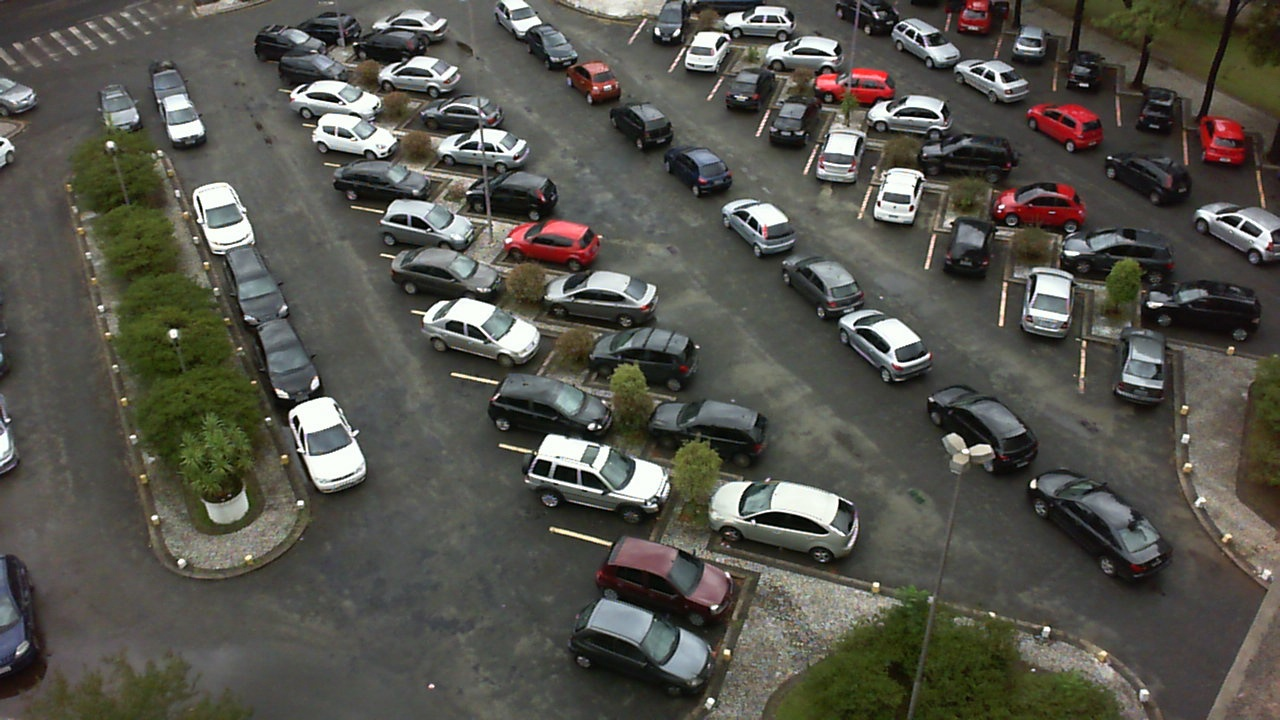
\includegraphics[width=110mm]{img/conception/pklot_park.jpg}
    \centering
    \caption{Image d'exemple provenant du dataset \textit{PKLot} qui sera utilisée afin de définir les divers paramètres}
    \label{fig:pklot-park}
\end{figure}


\paragraph{Sous-échantillonnage (\textit{Downsampling})}
Dans le but d'obtenir des images légères qu'un réseau de neurones peut traiter aisément et qu'aucune personne ou voiture ne puisse être reconnue, l'image est sous-échantillonnée. L'image peut être réduite à des tailles différentes: c'est ce qui sera testé dans cette section.

\paragraph{Détection de bord}
Il est possible de traiter les images en les filtrant à l'aide d'un filtre. Dans cette section, les matrices de convolutions suivantes, qui semblent donner les meilleurs résultats, ont été testées:
\begin{itemize}
    \item Sobel filter
    \item Scharr filter
\end{itemize} 

Il est important de noter que ces filtres ne peuvent être appliqué qu'à une image en valeurs de gris. Cependant, comme il a été défini en section \ref{techno.traitement.convolution} \itnameref{techno.traitement.convolution}, il est possible de séparer une image à 3 canaux en 3 images distinctes, d'effectuer le filtre sur chacun de ceux-ci, et de les recombiner en une image 3 canaux par la suite. 

Aussi, l'image a été convertie dans plusieurs représentations différentes, car en effet, les résultats obtenus peuvent en être modifiés. Les suivantes ont été testés:
\begin{description}
    \item[Valeur de gris] L'image peut être convertie en valeur de gris. En sortie, une image à un seul canal est produite.
    \item[RGB] L'image est représentée sous la forme de valeurs RGB de chacun des pixels. Elle est donc à 3 canaux, et les filtres seront appliqués sur chacun de ceux-ci.
    \item[HSV] L'image est convertie dans l'espace de couleur HSV. De la même manière que la représentation RGB, les 3 canaux résultants sont filtrés séparément.
\end{description}

Il est à noter que l'application d'un filtre de détection de bords a un grand rôle dans l'anonymisation des données, où des visages ou des modèles de voitures ne peuvent pratiquement pas être distingués dans les images en résultant.

\subsection{Evaluation des différentes méthodes et choix}
Dans cette section sont donc comparés différents filtres, résolutions et représentations d'images. 

Il faudra noter que le traitement peut être effectué de 2 manières différentes: soit l'image est premièrement sous-échantillonnée, soit les bords sont détectés. La méthodologie suivie afin de tester au mieux les différentes possibilités est la suivante:
\begin{enumerate}
    \item Les différentes possibilités de sous-échantillonnages et de détection de bords ont premièrement été explorés séparément.
    \item Le traitement "détection de bords en premier, suivi d'un sous-échantillonnage" a été testé.
    \item De la même manière, le traitement "sous-échantillonnage en premier, suivi d'une détection de bords" a lui aussi été exploré.
    \item Finalement, les deux traitements précisés en \textit{2} et \textit{3} ont été comparés.
\end{enumerate}

\paragraph{Sous-échantillonnage}\label{conception.traitement.eval.downsample}
Dans un premier temps, on comparera différentes résolutions d'images. Celles-ci sont les suivantes:
\begin{itemize}
    \item 1280 x 720 pixels
    \item 1120 x 630 pixels
    \item 960 x 540 pixels
    \item 800 x 450 pixels
    \item 640 x 360 pixels
    \item 480 x 270 pixels
    \item 320 x 180 pixels
    \item 160 x 90 pixels
\end{itemize}

\begin{figure}[H]
    \begin{subfigure}{.5\textwidth}
        \centering
        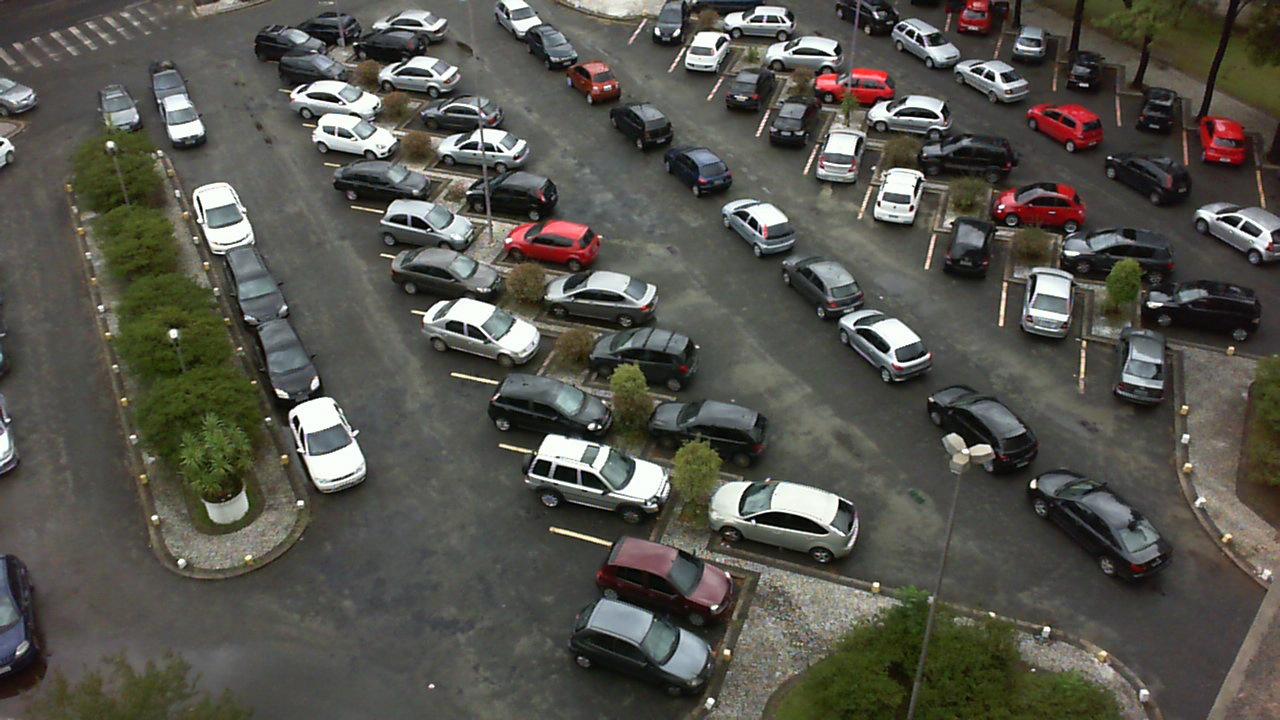
\includegraphics[width=.85\linewidth]{img/conception/image_process/downsample_only/7.png}
        \caption{1280 x 720}
    \end{subfigure}%
    \begin{subfigure}{.5\textwidth}
        \centering
        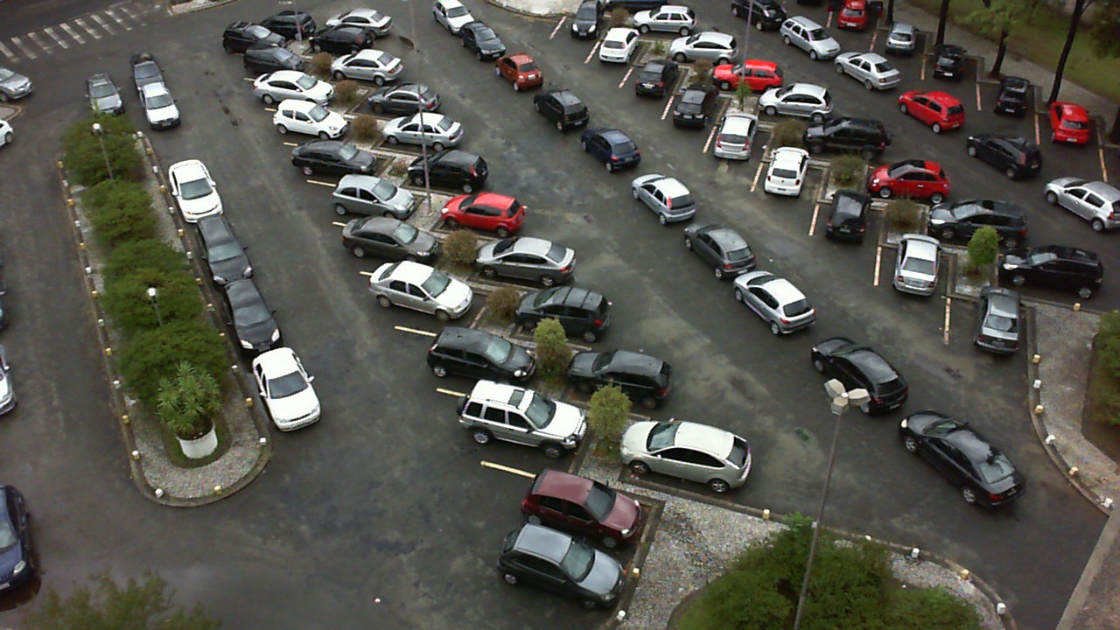
\includegraphics[width=.85\linewidth]{img/conception/image_process/downsample_only/6.png}
        \caption{1120 x 630}
    \end{subfigure}%   

    \bigskip
    \begin{subfigure}{.5\textwidth}
        \centering
        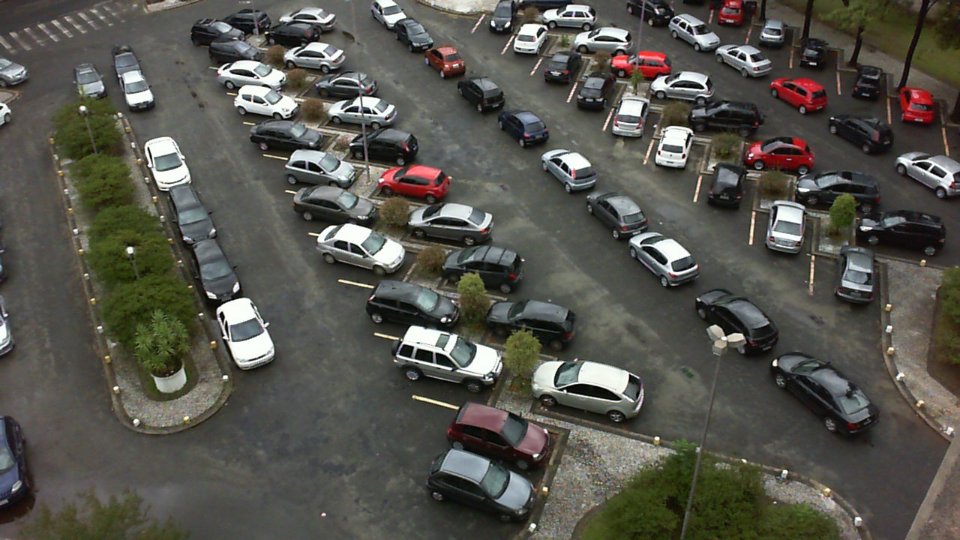
\includegraphics[width=.85\linewidth]{img/conception/image_process/downsample_only/5.png}
        \caption{960 x 540}   
    \end{subfigure}%   
    \begin{subfigure}{.5\textwidth}
        \centering
        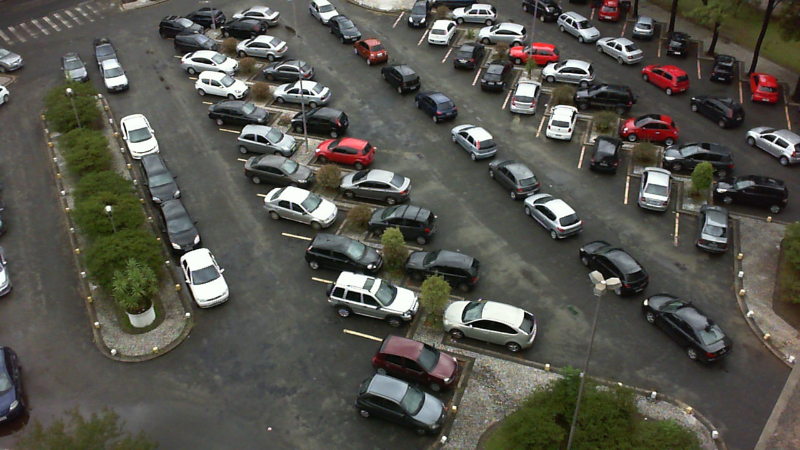
\includegraphics[width=.85\linewidth]{img/conception/image_process/downsample_only/4.png}
        \caption{800 x 450}
    \end{subfigure}% 

    \bigskip
    \begin{subfigure}{.5\textwidth}
        \centering
        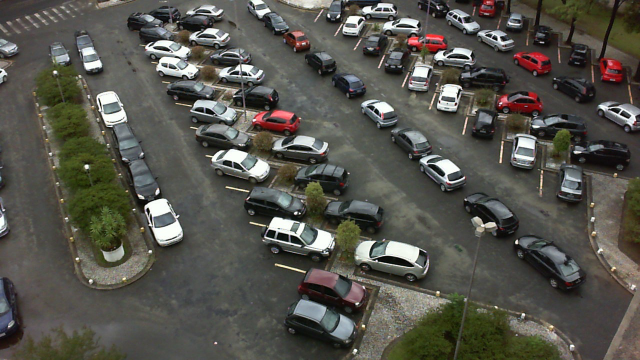
\includegraphics[width=.85\linewidth]{img/conception/image_process/downsample_only/3.png}
        \caption{640 x 360}
    \end{subfigure}%   
    \begin{subfigure}{.5\textwidth}
        \centering
        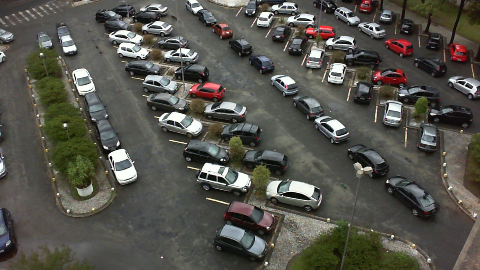
\includegraphics[width=.85\linewidth]{img/conception/image_process/downsample_only/2.png}
        \caption{480 x 270}
    \end{subfigure}%  
    
    \bigskip
    \begin{subfigure}{.5\textwidth}
        \centering
        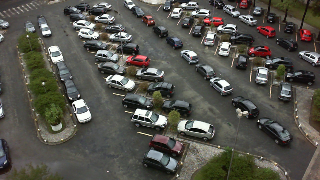
\includegraphics[width=.85\linewidth]{img/conception/image_process/downsample_only/1.png}
        \caption{320 x 180}
    \end{subfigure}%   
    \begin{subfigure}{.5\textwidth}
        \centering
        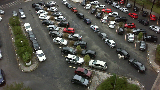
\includegraphics[width=.85\linewidth]{img/conception/image_process/downsample_only/0.png}
        \caption{160 x 90}
    \end{subfigure}%   
    \centering
    \caption{L'image originale redimensionnée à différentes résolutions}
    \label{fig:image_process_downsampling}
\end{figure}

On trouvera en figure \ref{fig:image_process_downsampling} les résultats du rééchantillonnage en fonction des diverses résolutions.

Il semble que la résolution de 320x180 pixel soit suffisante à bien distinguer les voitures. Cependant, on notera que celle-ci pourrait ne pas l'être après application du filtre de détection de contours.

\paragraph{Détection de bords}

Les filtres \textit{Sobel} et \textit{Scharr}, ainsi que les représentations RGB, HSV et en valeurs de gris ont été testés. La figure \ref{fig:image_process_edges} en montre les résultats si ces filtres sont appliqués sur l'images originales. Sur celle-ci, on distinguera les 2 filtres par les colonnes, et les 3 représentations par les lignes.

\begin{figure}[H]
    \begin{subfigure}{.5\textwidth}
        \centering
        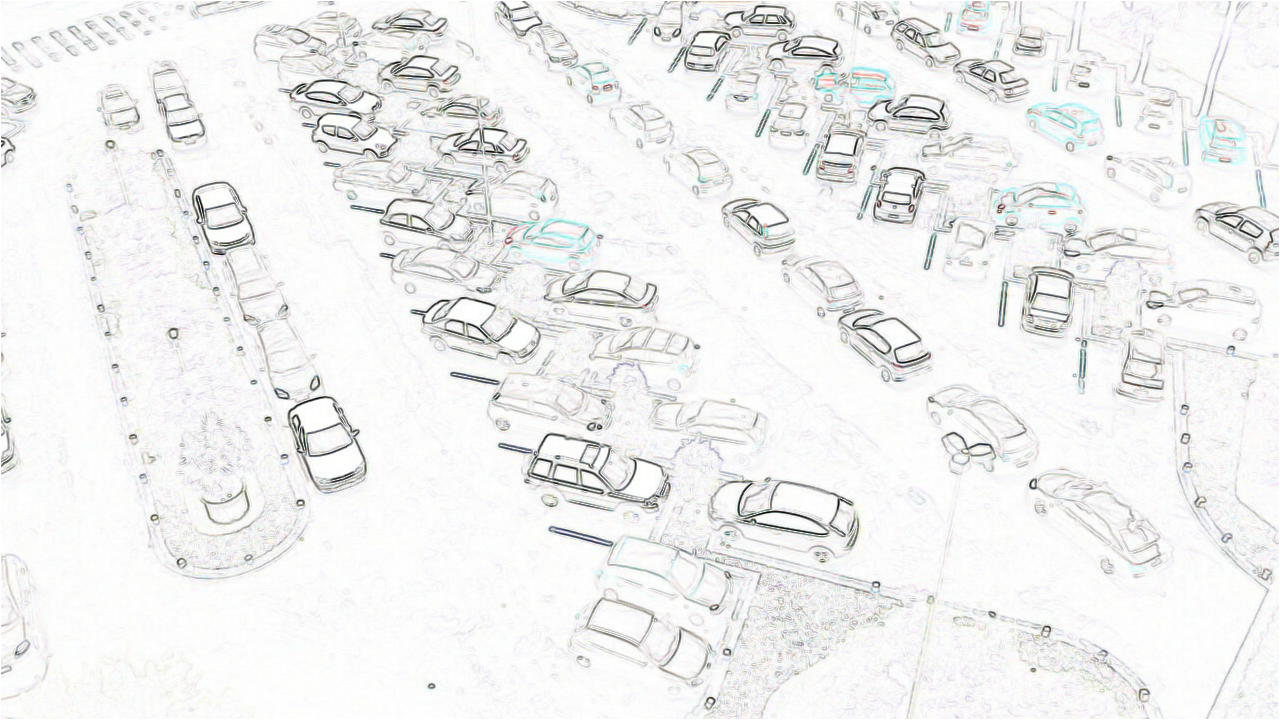
\includegraphics[width=.85\linewidth]{img/conception/image_process/edges_only/0.png}
        \caption{Filtre \textit{Sobel} - RGB}
    \end{subfigure}%   
    \begin{subfigure}{.5\textwidth}
        \centering
        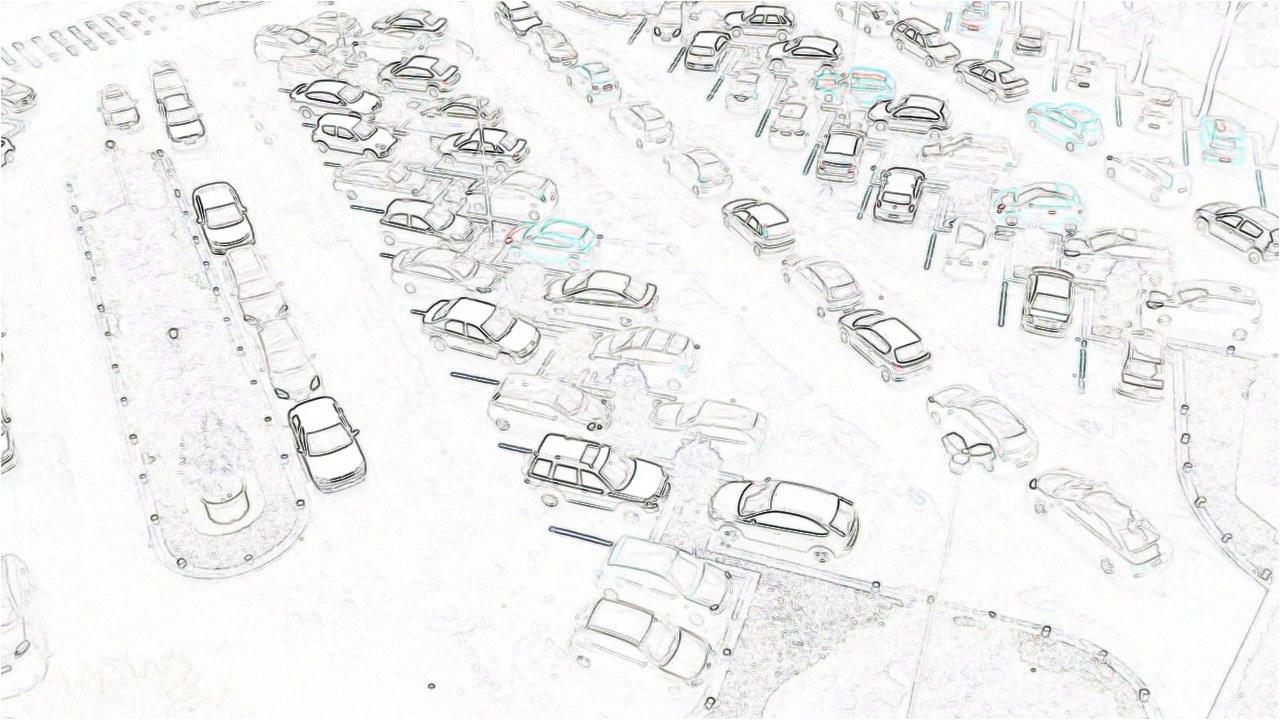
\includegraphics[width=.85\linewidth]{img/conception/image_process/edges_only/3.png}
        \caption{Filtre \textit{Scharr} - RGB}
    \end{subfigure}%  

    \bigskip
    \begin{subfigure}{.5\textwidth}
        \centering
        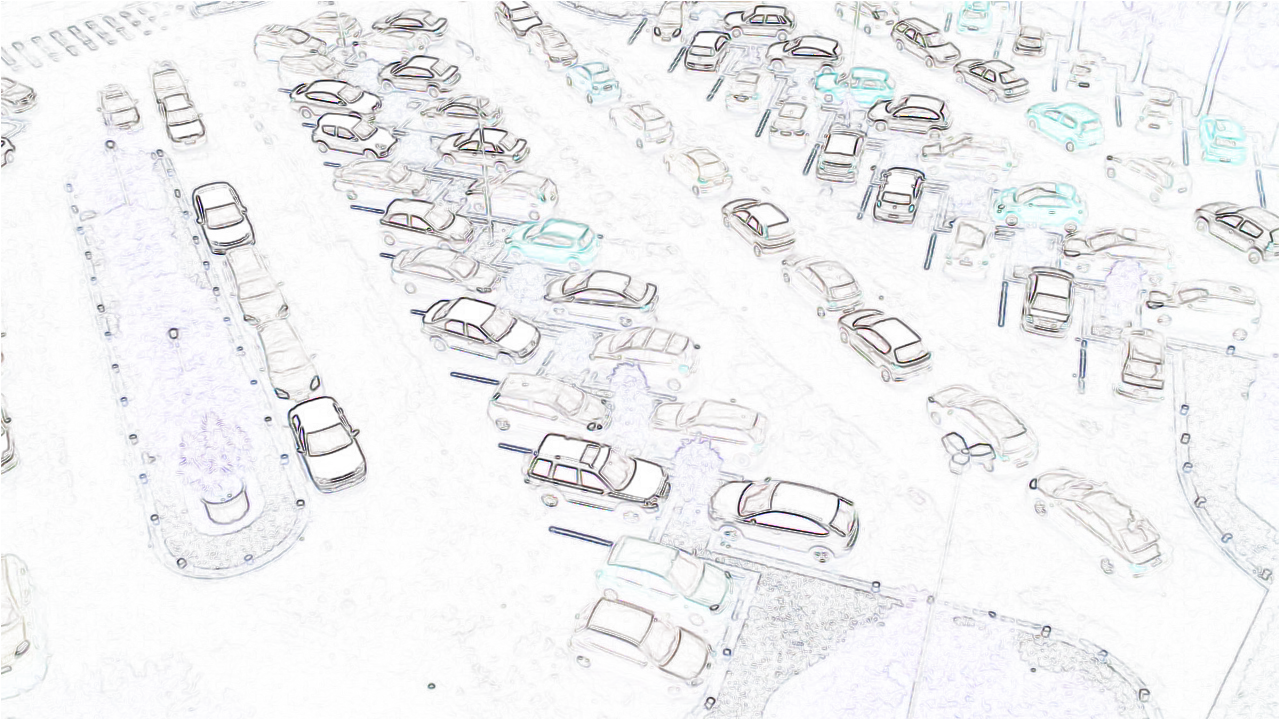
\includegraphics[width=.85\linewidth]{img/conception/image_process/edges_only/1.png}
        \caption{Filtre \textit{Sobel} - HSV}   
    \end{subfigure}%   
    \begin{subfigure}{.5\textwidth}
        \centering
        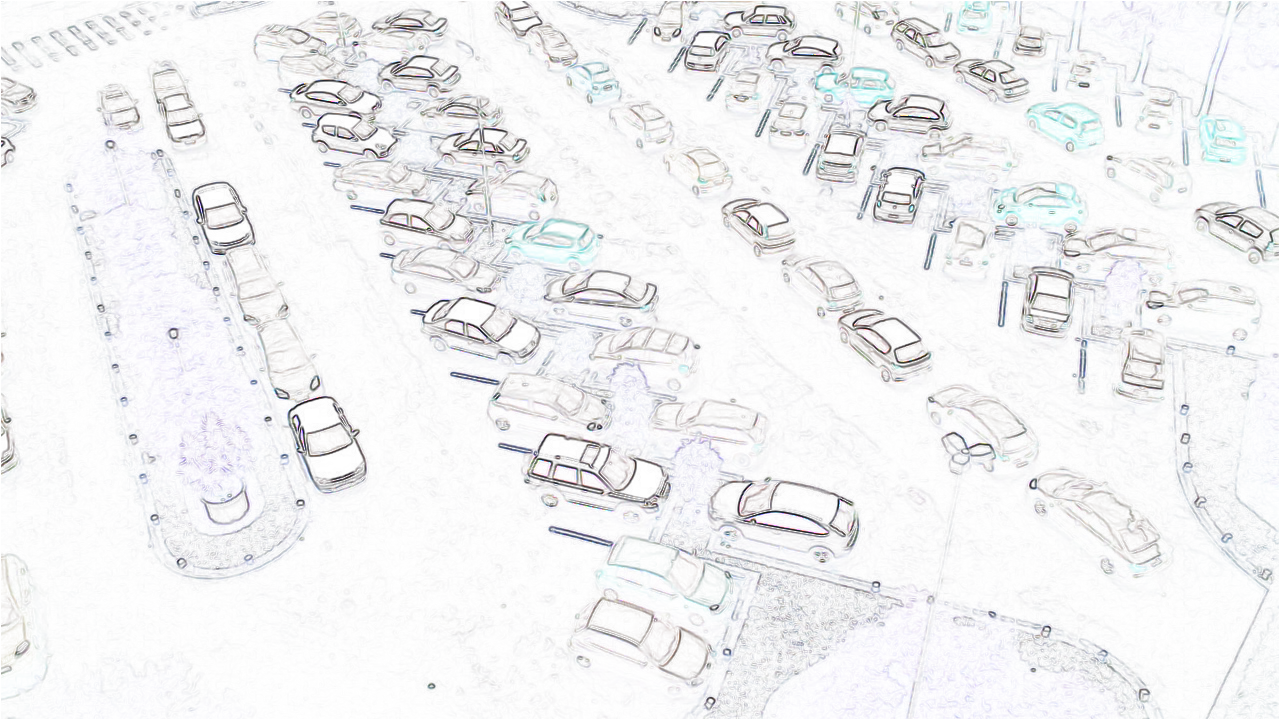
\includegraphics[width=.85\linewidth]{img/conception/image_process/edges_only/4.png}
        \caption{Filtre \textit{Scharr} - HSV}
    \end{subfigure}% 
    
    \bigskip
    \begin{subfigure}{.5\textwidth}
        \centering
        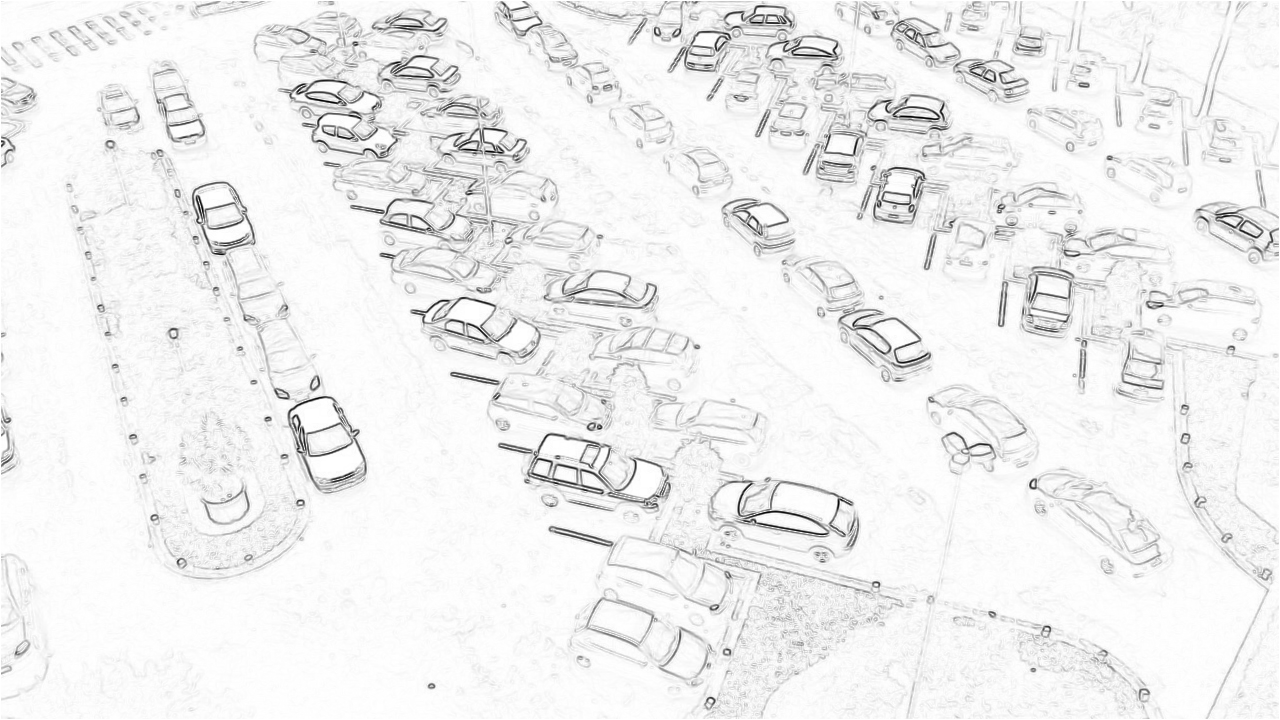
\includegraphics[width=.85\linewidth]{img/conception/image_process/edges_only/2.png}
        \caption{Filtre \textit{Sobel} - Valeurs de gris}
    \end{subfigure}%   
    \begin{subfigure}{.5\textwidth}
        \centering
        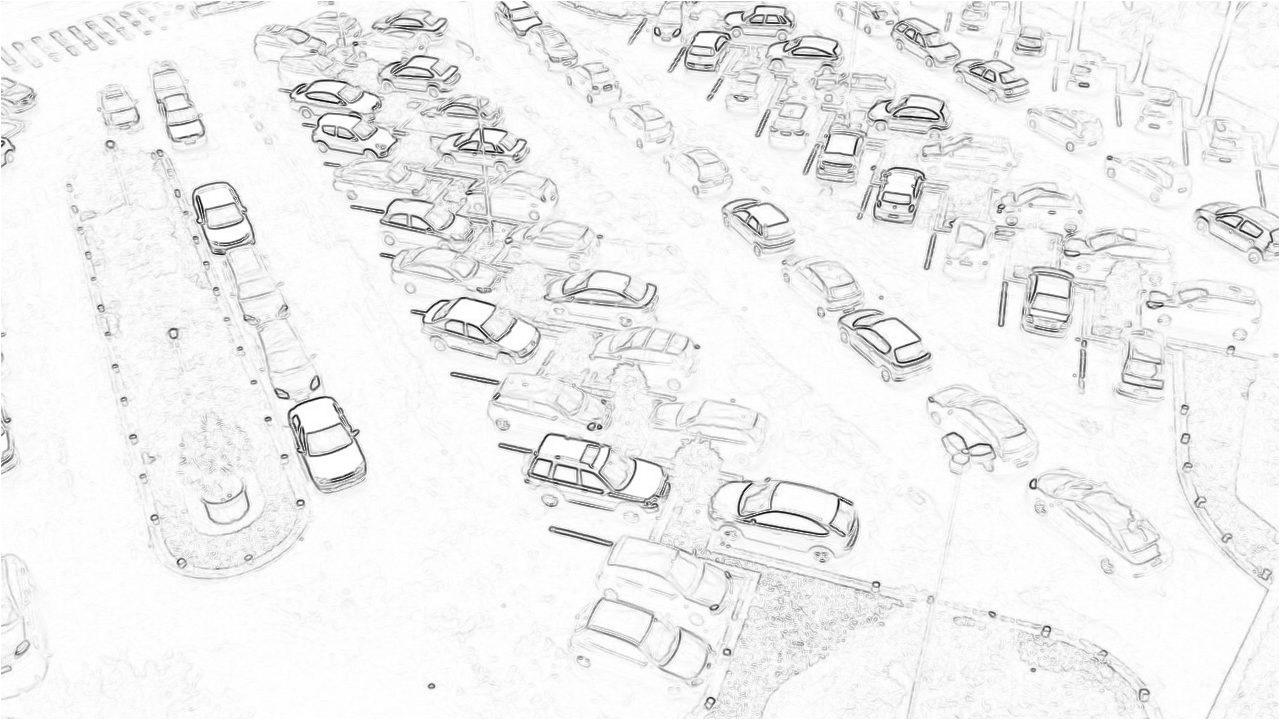
\includegraphics[width=.85\linewidth]{img/conception/image_process/edges_only/5.png}
        \caption{Filtre \textit{Scharr} - Valeurs de gris}
    \end{subfigure}%   
    \centering
    \caption{L'image originale avec différentes détections de bords}
    \label{fig:image_process_edges}
\end{figure}

Les résultats sont assez similaires. Evidemment, la représentation en valeurs de gris fait perdre toutes notions de couleur. Entre les deux autres représentations, on peut remarquer que l'espace HSV permet de plus facilement distinguer les différentes couleurs. Celles-ci ont leurs importances dans ce projet: en effet, une voiture rouge est facilement distinguable de l'herbe verte. 

Concernant les deux filtres \textit{Sobel} et \textit{Scharr}, il n'y a que très peu de différences. Cependant, il semble que la matrice de convolution de \textit{Scharr} offre une détection de bords légèrement meilleure.

Ainsi, un filtre \textit{Scharr} appliqué sur l'espace de couleur \textit{HSV} semble le plus indiqué. Il faut noter que ceci peut dépendre du sous-échantillonnage. Concernant l'espace de couleur HSV, si celui-ci ne convient pas pour le \textit{Machine Learning}, il sera toujours possible de convertir les images en valeurs de gris.

\paragraph{Détection de bords, sous-échantillonnage}
Ici, il est considéré que la détection de bord a été effectuée en premier. Celle-ci correspond au paragraphe précédent: un filtre \textit{Scharr} est appliqué sur l'espace HSV de l'image.

\begin{figure}[H]
    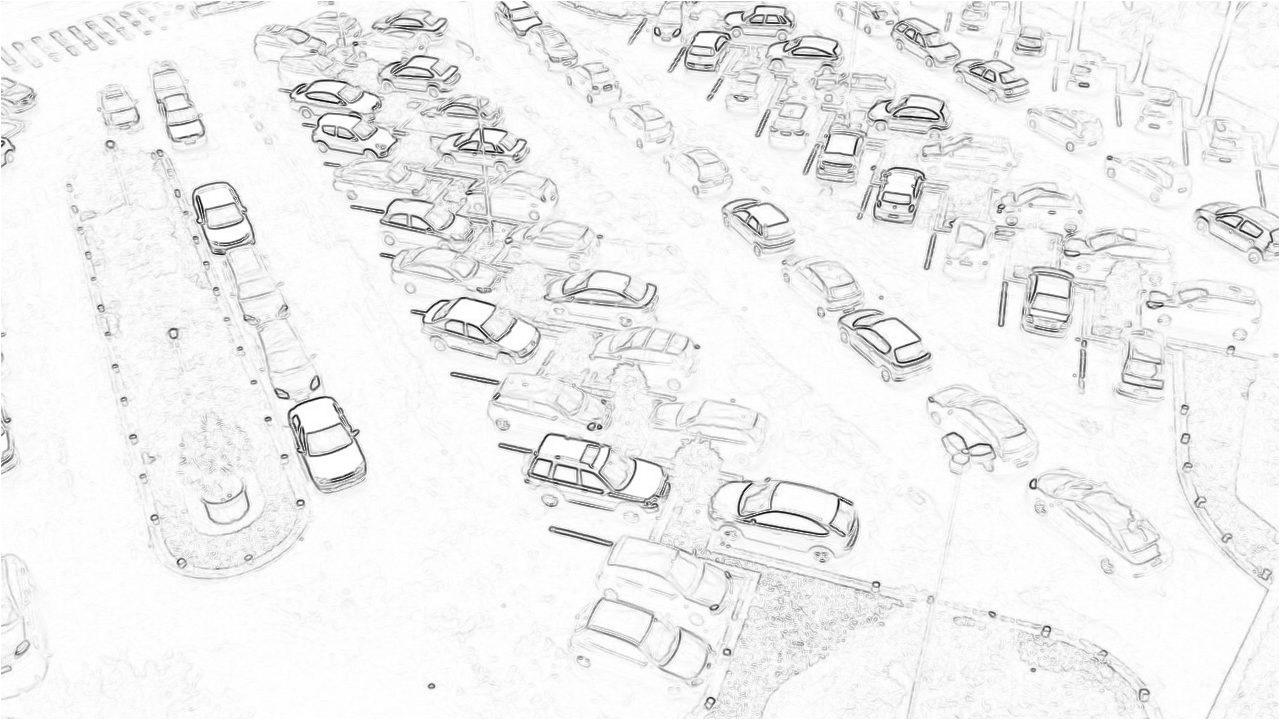
\includegraphics[width=110mm]{img/conception/image_process/edges_only/5.png}
    \centering
    \caption{\textit{Scharr} HSV: image utilisée afin d'explorer les différents sous-échantillonnages}
    \label{fig:image_process_edge_down_orig}
\end{figure}

\begin{figure}[H]
    \begin{subfigure}{.5\textwidth}
        \centering
        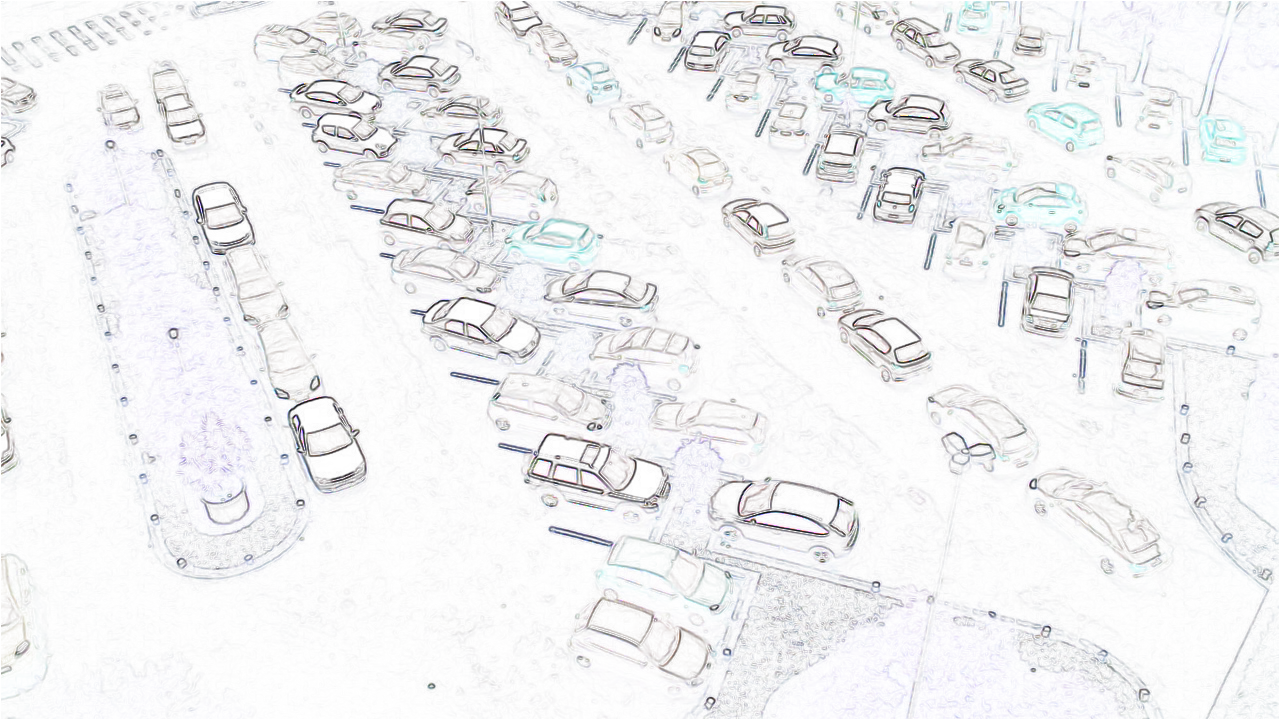
\includegraphics[width=.85\linewidth]{img/conception/image_process/edge-downsample/7.png}
        \caption{1280 x 720}
    \end{subfigure}%
    \begin{subfigure}{.5\textwidth}
        \centering
        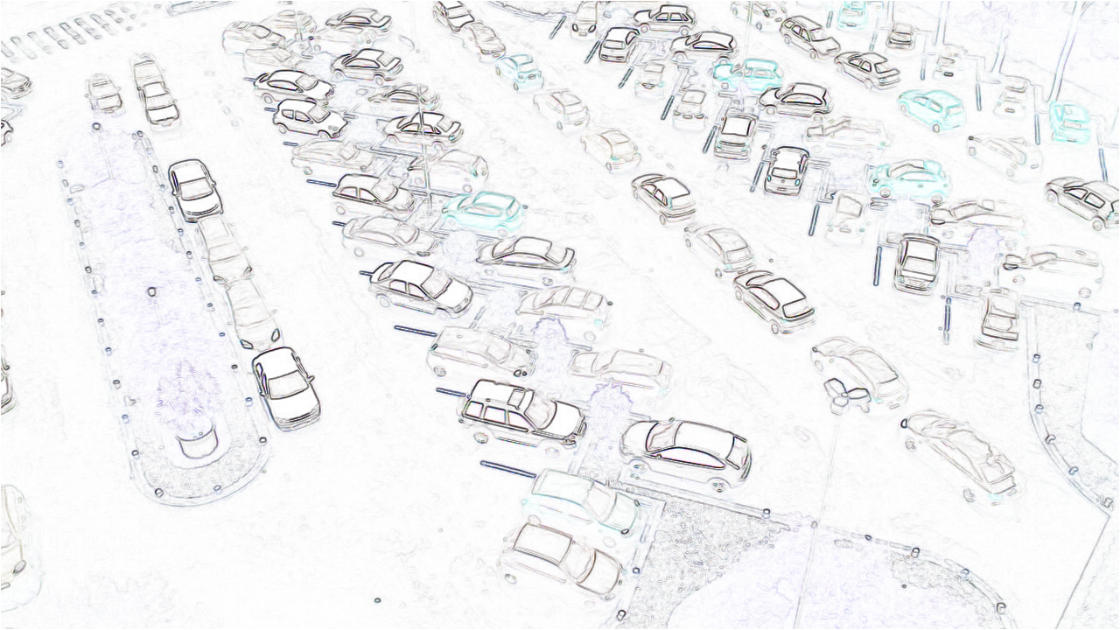
\includegraphics[width=.85\linewidth]{img/conception/image_process/edge-downsample/6.png}
        \caption{1120 x 630}
    \end{subfigure}%   

    \bigskip
    \begin{subfigure}{.5\textwidth}
        \centering
        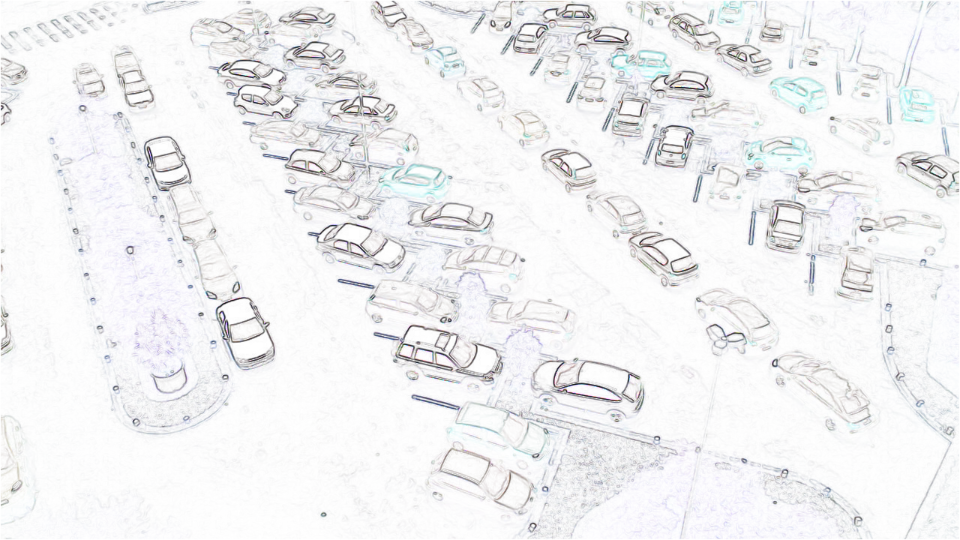
\includegraphics[width=.85\linewidth]{img/conception/image_process/edge-downsample/5.png}
        \caption{960 x 540}   
    \end{subfigure}%   
    \begin{subfigure}{.5\textwidth}
        \centering
        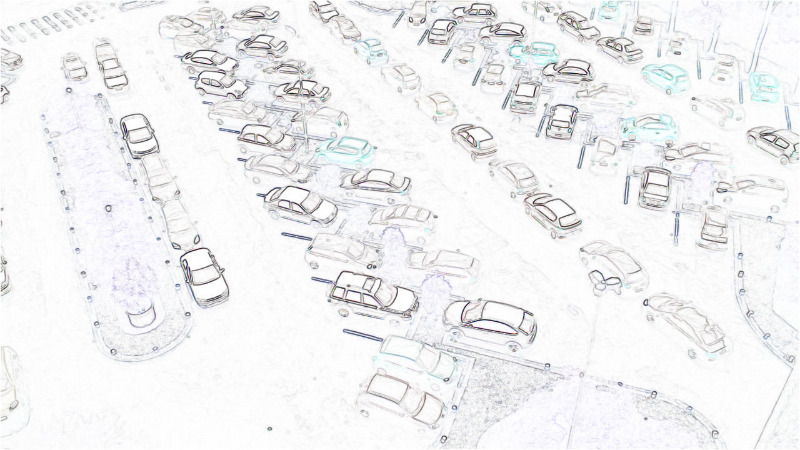
\includegraphics[width=.85\linewidth]{img/conception/image_process/edge-downsample/4.png}
        \caption{800 x 450}
    \end{subfigure}% 

    \bigskip
    \begin{subfigure}{.5\textwidth}
        \centering
        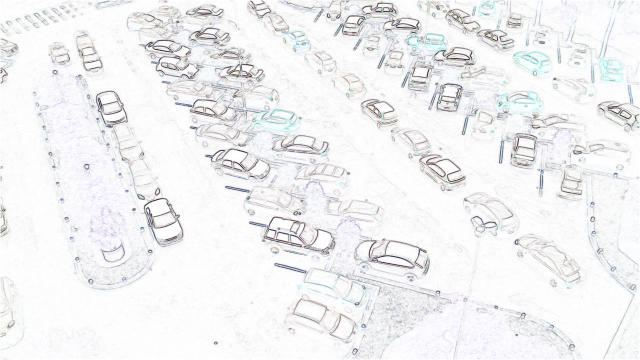
\includegraphics[width=.85\linewidth]{img/conception/image_process/edge-downsample/3.png}
        \caption{640 x 360}
    \end{subfigure}%   
    \begin{subfigure}{.5\textwidth}
        \centering
        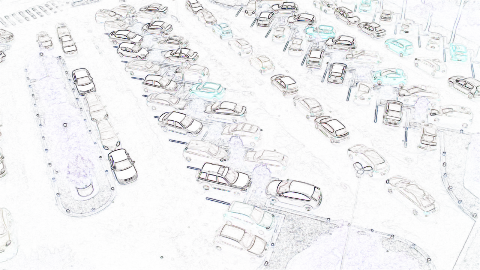
\includegraphics[width=.85\linewidth]{img/conception/image_process/edge-downsample/2.png}
        \caption{480 x 270}
    \end{subfigure}%  
    
    \bigskip
    \begin{subfigure}{.5\textwidth}
        \centering
        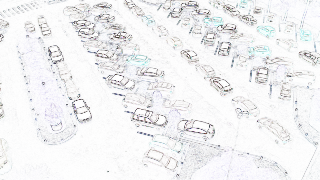
\includegraphics[width=.85\linewidth]{img/conception/image_process/edge-downsample/1.png}
        \caption{320 x 180}
    \end{subfigure}%   
    \begin{subfigure}{.5\textwidth}
        \centering
        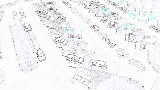
\includegraphics[width=.85\linewidth]{img/conception/image_process/edge-downsample/0.png}
        \caption{160 x 90}
    \end{subfigure}%   
    \centering
    \caption{L'image dont les bords ont été détectés, redimensionnée à différentes résolutions}
    \label{fig:image_process_edge_down}
\end{figure}

La figure \ref{fig:image_process_edge_down} applique plusieurs sous-échantillonnages de l'image \ref{fig:image_process_edge_down_orig}.

Il semble que l'image la plus légère et suffisamment précise afin de pouvoir détecter sans encombre des voitures est celle dont la résolution est de 480 x 270 pixels. Les images dont la taille est inférieure sont trop floues, où certaines voitures semblent parfois même disparaitre.

\paragraph{Sous-échantillonnage, détection de bords}\label{conception.traitement.eval.down-edge}
Ce paragraphe présente les résultats d'un traitement qui consiste en sous-échantillonner l'image dans un premier temps, puis d'en détecter les bords. Lors des différents tests effectués, il a été remarqué qu'une résolution de 320x180 pixels, tel qu'indiqué dans le paragraphe \itnameref{conception.traitement.eval.downsample}, ne produisait pas des résultats concluants. C'est pourquoi la résolution de 480 x 270 pixels a été préférée. L'image utilisée est présentée en figure \ref{fig:image_process_down_edge_orig}.

\begin{figure}[H]
    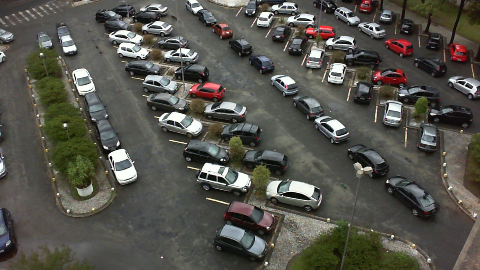
\includegraphics[width=110mm]{img/conception/image_process/downsample_only/2.png}
    \centering
    \caption{480 x 270: image utilisée afin d'explorer les différentes méthodes de détection de bords}
    \label{fig:image_process_down_edge_orig}
\end{figure}

\begin{figure}[H]
    \begin{subfigure}{.5\textwidth}
        \centering
        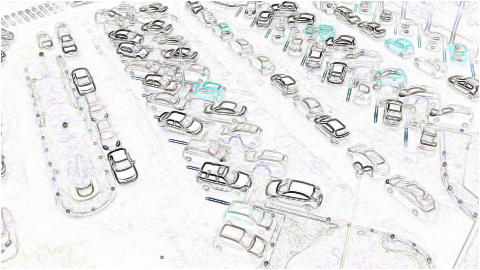
\includegraphics[width=.85\linewidth]{img/conception/image_process/downsample-edge/0.png}
        \caption{Filtre \textit{Sobel} - RGB}
    \end{subfigure}%   
    \begin{subfigure}{.5\textwidth}
        \centering
        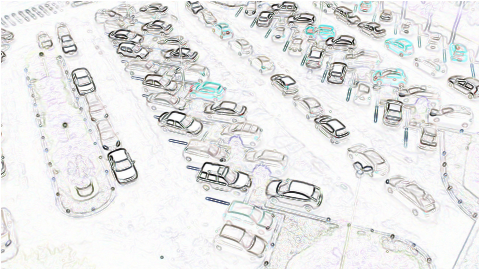
\includegraphics[width=.85\linewidth]{img/conception/image_process/downsample-edge/3.png}
        \caption{Filtre \textit{Scharr} - RGB}
    \end{subfigure}%  

    \bigskip
    \begin{subfigure}{.5\textwidth}
        \centering
        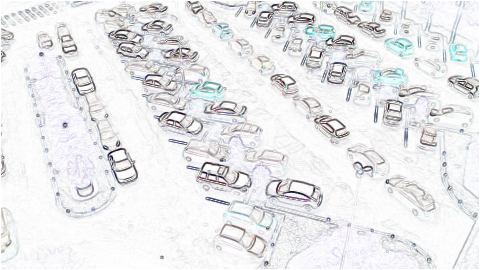
\includegraphics[width=.85\linewidth]{img/conception/image_process/downsample-edge/1.png}
        \caption{Filtre \textit{Sobel} - HSV}   
    \end{subfigure}%   
    \begin{subfigure}{.5\textwidth}
        \centering
        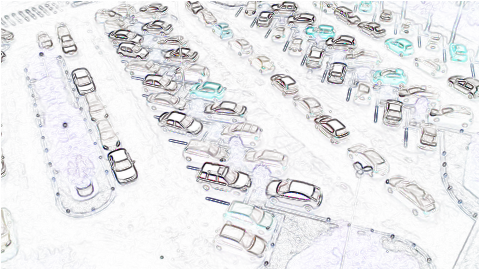
\includegraphics[width=.85\linewidth]{img/conception/image_process/downsample-edge/4.png}
        \caption{Filtre \textit{Scharr} - HSV}
    \end{subfigure}% 
    
    \bigskip
    \begin{subfigure}{.5\textwidth}
        \centering
        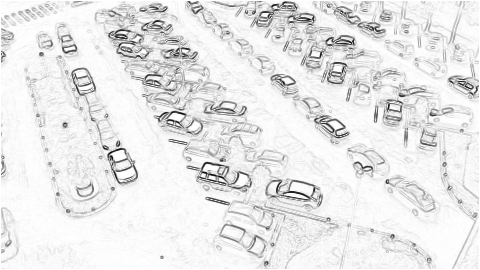
\includegraphics[width=.85\linewidth]{img/conception/image_process/downsample-edge/2.png}
        \caption{Filtre \textit{Sobel} - Valeurs de gris}
    \end{subfigure}%   
    \begin{subfigure}{.5\textwidth}
        \centering
        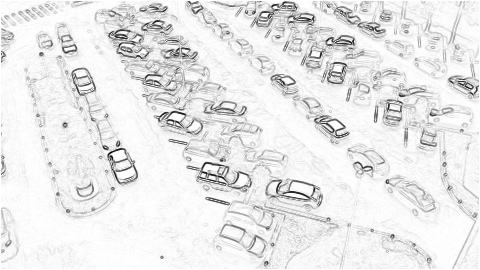
\includegraphics[width=.85\linewidth]{img/conception/image_process/downsample-edge/5.png}
        \caption{Filtre \textit{Scharr} - Valeurs de gris}
    \end{subfigure}%   
    \centering
    \caption{L'image sous-échantillonnée avec différentes détections de bords}
    \label{fig:image_process_down_edge}
\end{figure}

La figure \ref{fig:image_process_down_edge} présente l'application des différents filtres sur l'image sous-échantillonnées

Ici, de la même manière que décrit au paragraphe \itnameref{conception.traitement.eval.down-edge}, le filtre semblant le mieux convenir est la matrice de convolution définie par \textit{Scharr} sur l'espace HSV. Les voitures y sont mieux distinguables, notamment grâce à leurs couleurs.

\paragraph{Comparaison des deux méthodes de traitement}

Il est maintenant possible de comparer les deux méthodes de traitement définies aux deux derniers paragraphes. La figure \ref{fig:image_process_compare} présente leur résultat côte-à-côte.

\begin{figure}[H]
    \begin{subfigure}{\textwidth}
        \centering
        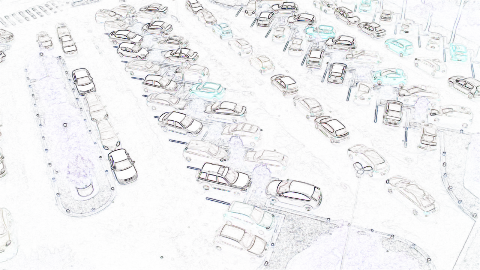
\includegraphics[width=.8\linewidth]{img/conception/image_process/edge-downsample/2.png}
        \caption{Ici, les bords de l'images ont été détectés, puis celle-ci a été réduite à une taille de 480 x 270 pixels}
    \end{subfigure}%   

    \bigskip
    \begin{subfigure}{\textwidth}
        \centering
        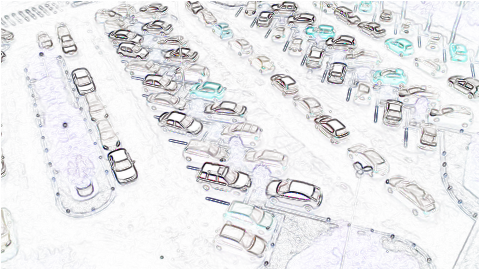
\includegraphics[width=.8\linewidth]{img/conception/image_process/downsample-edge/4.png}
        \caption{Filtre \textit{Scharr} - RGB}
    \end{subfigure}%    
    \centering
    \caption{Ici, l'image a premièrement été réduite à une taille de 480 x 270 pixels, puis les bords ont été détectés}
    \label{fig:image_process_compare}
\end{figure}

La différence principale entre ces deux images réside dans les bords détectés, où la méthode \textit{b} permet de les mettre plus en valeur. Les traits sont plus foncés et épais. Certaines voitures sont moins distinguables dans la méthode \textit{a}, se fondant dans le fond.

Il sera donc possible de résumer le traitement qui sera effectué sur l'image de la manière suivante:
\begin{enumerate}
    \item L'image sera réduite à une taille de 480 x 270 pixels
    \item Un filtre \textit{Scharr} sera appliqué sur chacun des canaux de l'espace HSV de cette image.
\end{enumerate}

\todo{Réduire détection de bord, en annexe ?}

\section{Conception des modèles}

Cette section permet les solutions qui ont été pensées pour résoudre le problème de détection du taux d'utilisation du parking. Le modèle final choisi et aussi présenté. 

\subsection{Suppression d'arrière-plan}

\todo{AOSäDHJ OPIAHJDPüASD }

\subsection{Regression}\label{conception.model.regression}
La première approche qui a été pensée est d'aborder le problème comme une simple regression.

Un tel problème consiste en une fonction dont la sortie est quantitative, et non qualitative\autocite{wiki:regression}. Dans notre cas, cela signifie qu'en sortie de l'algorithme, on cherche le nombre de voitures présentes sur l'image présentée en entrée. 

Pour ce faire, un réseau de neurones à convolutions, comme décrit en section \ref{techno.nn.convolution} \itnameref{techno.nn.convolution} peut être utilisé. 

On trouvera en figure \ref{fig:regression_keras} un modèle qui peut être utilisé, et qui a été testée. Le schéma se lit de haut en bas, de la couche d'entrée à la couche de sortie. Ce modèle a été défini à l'aide de la librairie \textit{Keras}

\begin{figure}[H]
    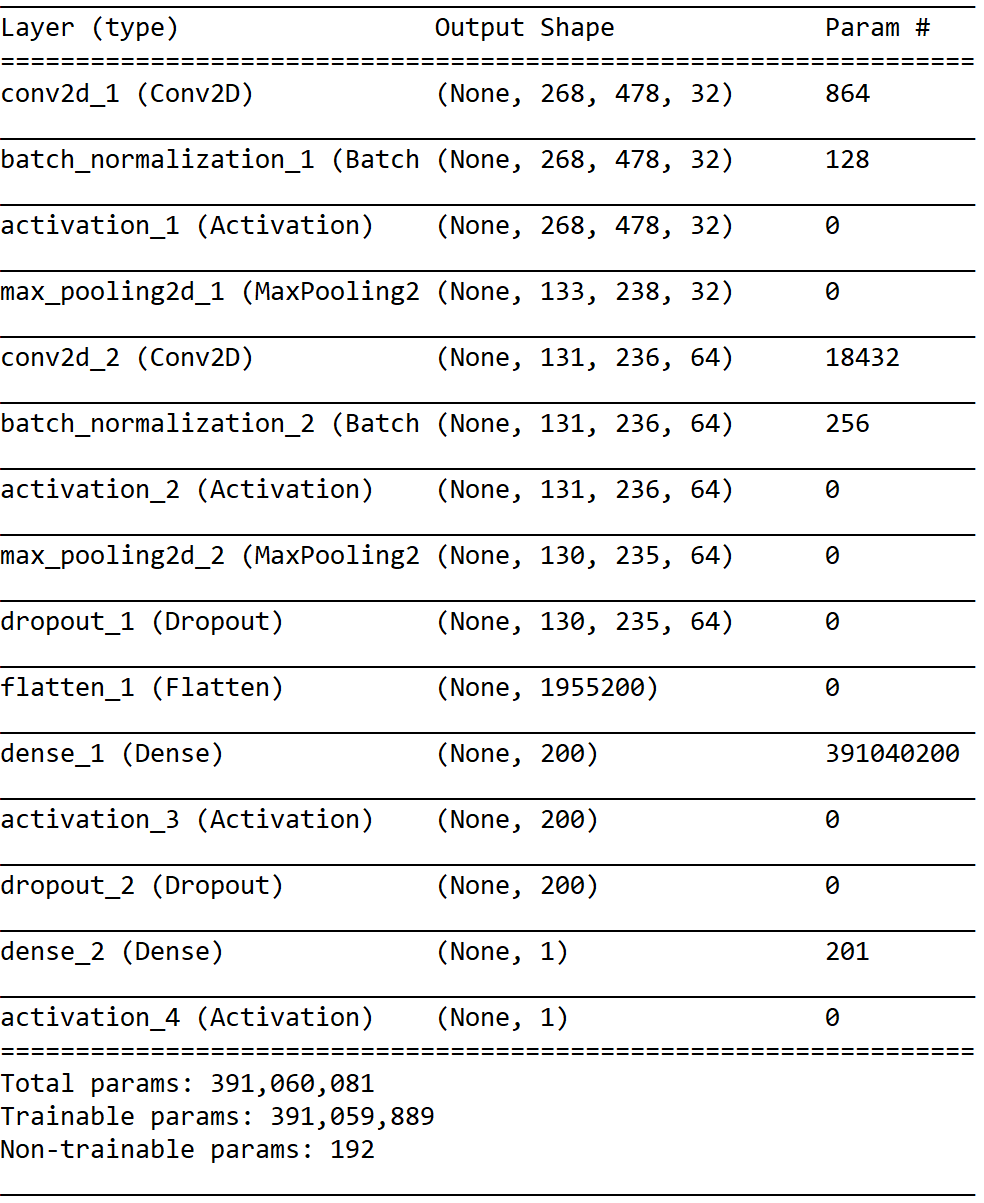
\includegraphics[width=12cm]{img/conception/nn/regression_keras.png}
    \centering
    \caption{Proposition de modèle de réseau de neurones à convolutions pour résoudre le problème de regression}
    \label{fig:regression_keras}
\end{figure} 

En entrée, une image de parking est passée, qui sont traitée par une première couche de convolutions. En sortie, un simple neurone permet d'indiquer le nombre total de voiture présentes sur l'image. 


Il est aussi possible d'y remarquer une succession de couches telles que les suivantes:

\begin{description}
    \item[\textit{Batch normalization}] permet de normaliser les données, dans le but d'accélérer l'apprentissage.
    \item[\textit{Max pooling}] permet de réduire la taille des images en entrée.\footnote{C'est une méthode classique utilisées dans les réseaux de neurones convolutifs. En effet, une telle couche de \textit{max pooling} est généralement présente après une couche de convolutions. \autocite{wiki:CNN}} 
    \item[\textit{Activation}] la couche des fonctions d'activations \footnote{Une fonction d'activation est généralement associée à chaque neurones dans les réseaux neuronaux \autocite{wiki:NN}}. 
    \item[\textit{Flatten}] d'images en entrée (tenseur\footnote{Un tenseur peut être comparé à un tableau à n dimension. Un tenseur à 2 dimension est tous simplement une matrice. } à 2 dimensions), cette couche permet de les aplatir en un tenseur à 1 dimension, nécessaire en entrée d'un réseau de neurones classique.
    \item[\textit{Dropout}] permet de mieux généraliser. Certaines relations entre les neurones de deux couches sont simplement supprimées.
    \item[\textit{Dense}] ajoute une couche de neurones classiques. 
\end{description}

Il faut noter que les données de sortie a été normalisée dans le but d'accélérer l'entrainement. Ainsi, la sortie, plutôt que d'indiquer le nombre de véhicule, indique le taux d'utilisation du parking, entre $0$ et $1$. Cette valeur peut être facilement calculée lorsqu'on connait le nombre maximal de voitures qui peuvent y être présentes. La fonction suivante permet de le calculer, où $v$ est le nombre de voitures présentes, et $c$ la capacité du parking:
\[
    f(v) = \frac{vente}{c}
\]

Les diverses fonctions d'activations ne sont pas présentées sur la figure \ref{fig:regression_keras}. Deux différentes ont été utilisées:

\begin{description}
    \item[\textit{Relu} (\textit{Rectified Linear Unit})] Simple fonction linéaire qui transforme les valeurs négatives en entrée en $0$ en sortie. Très souvent utilisée dans les réseaux de neurones à convolutions. Toutes les fonctions d'activations présentes, mis à part celle de sortie, sont une \textit{Relu}.
    \item[\textit{Sigmoïde}] Fonction d'activation qui transforme les valeurs d'entrée en une valeur de sortie entre 0 et 1. Elle est utilisée en sortie, ce qui permet d'obtenir le taux d'occupation du parking aisément.
\end{description}

Il faut noter que le modèle présenté n'en est qu'un parmi plusieurs autres qui ont été testés. Cependant, les résultats finaux n'ont pas été concluants, et il ne sera pas plus amplement exploré dans ce rapport. Il est cependant possible d'émettre quelques hypothèses pouvant expliquer ces disfonctionnements:

\begin{itemize}
    \item Le problème à résoudre peut ne pas être si simple. Un réseau de neurones plus complexe, en multipliant le nombre de couches, doit sans doute être nécessaires. 
    \item Le label \textit{taux d'utilisation du parking} ne donne au réseau de neurones aucune indication sur ce qu'il doit prendre en compte et distinguer dans les images. Indiquer où sont les voitures peut sembler plus efficaces.
    \item Le nombre d'itérations effectuées lors des tests peut être trop faible. En effet, lorsqu'on observe ce qui est fait dans le domaine de la détection d'objet, plusieurs dizaines d'itérations sont en générales effectuées. 
\end{itemize}

\subsection{Grille de détection} 
Le modèle précédent décrit en section \ref{conception.model.regression} n'a pas permis d'obtenir de résultats concluant. Il a notamment été précisé qu'une indication concernant la position des voitures semblait pouvoir permettre d'améliorer les résultats. De part cette hypothèse, il a été pensé qu'il est sans doute possible de chercher à obtenir en sortie de l'algorithme la position des voitures plutôt que leur nombre.

Pour ce faire, il a été pensé de subdiviser l'image d'entrée en une grille. Cette idée est inspirée par ce qui est fait dans l'algorithme \textit{Yolo}, décrit en section \ref{techno.nn.object}. La figure \ref{fig:parking_grid} présente une subdivision de \textit{5x4} sur une image de parking. En chaque cellule de la grille, on cherchera à savoir si une voiture y est présente. 

\begin{figure}[ht]
    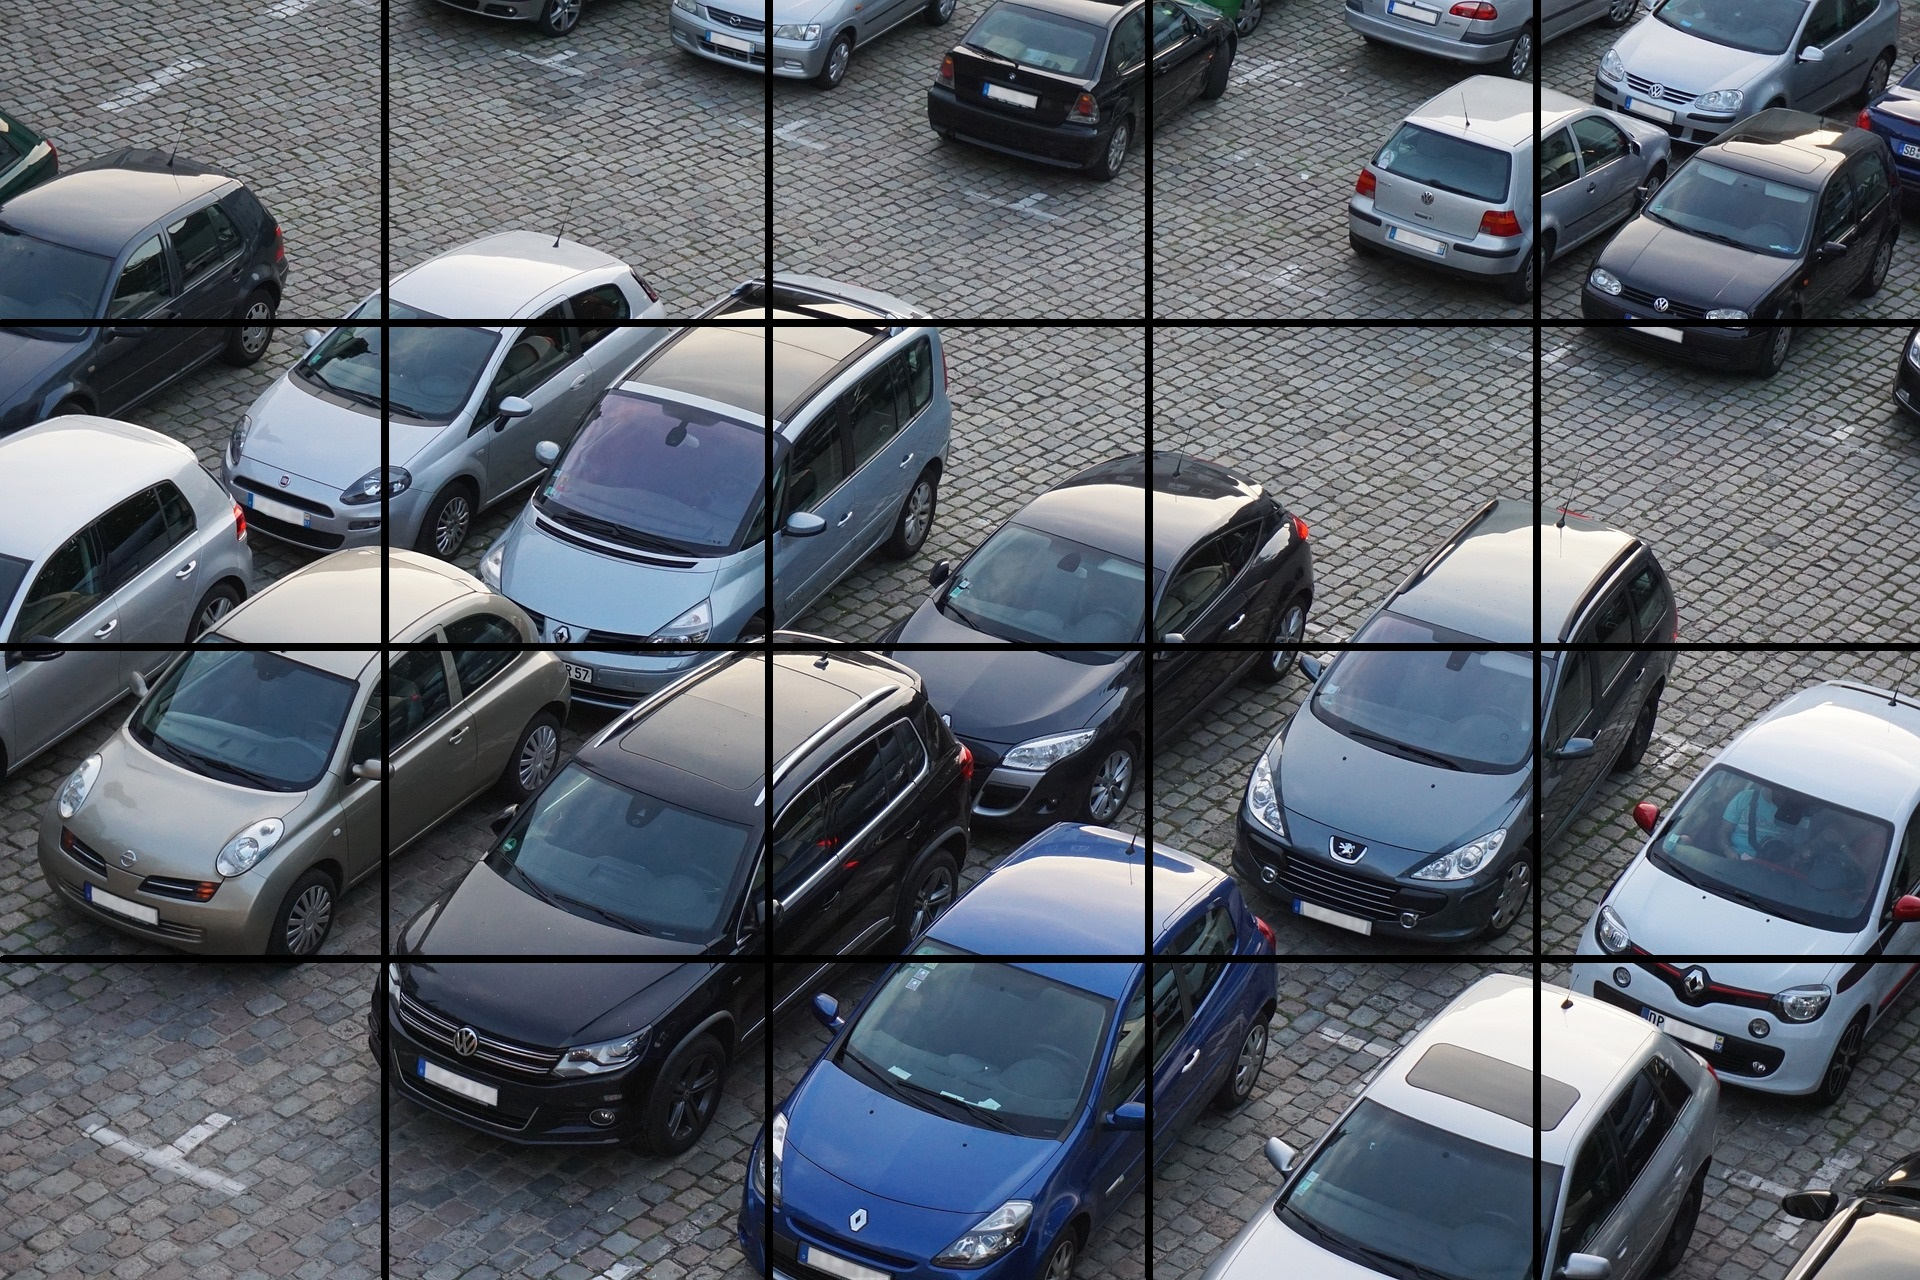
\includegraphics[width=120mm]{img/conception/parking_grid.jpg}
    \centering
    \captionsource{Image de parking subdivisée selon une grille}{img:parking}
    \label{fig:parking_grid} 
\end{figure}

Il faut noter qu'une cellule contient une voiture seulement si le centre de l'objet y est présent. Ainsi, chaque voiture est détectée une seule fois. Aussi, la grille présentée en figure \ref{fig:parking_grid} a une faible dimension, où il est possible qu'une cellule contienne deux voitures. En réalité, la grille doit avoir des dimensions supérieures à \textit{5x4}.

\begin{figure}[H]
    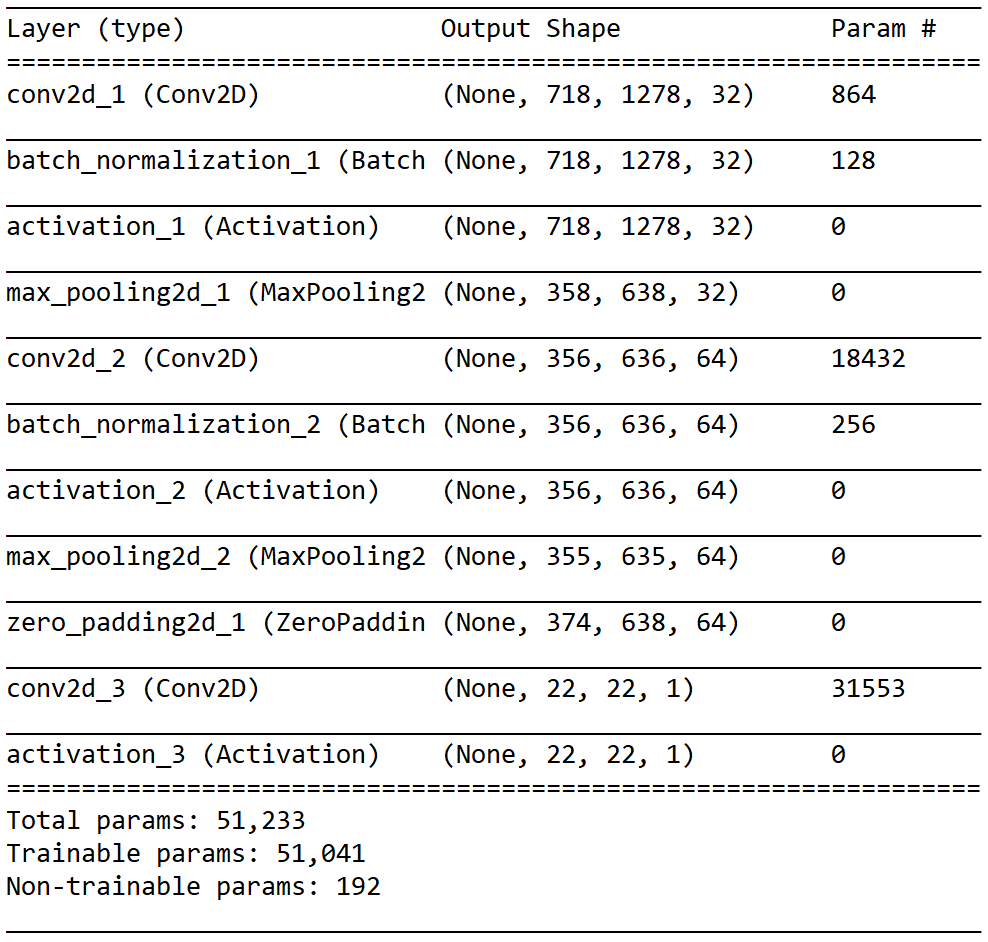
\includegraphics[width=12cm]{img/conception/nn/keras_grid.png}
    \centering
    \caption{Proposition de modèle de réseau de neurones à convolutions, avec une grille en sortie}
    \label{fig:keras_grid}
\end{figure} 

La figure \ref{fig:keras_grid} présente un modèle de réseau de neurones. Celui-ci reprends principalement le modèle développé précédemment en section \ref{conception.model.regression} \itnameref{conception.model.regression}. On remarque cependant que la sortie diffère: en lieu et place d'un unique neurone de sortie, un tensor 2D y est présent. Chaque cellule de ce tableau peut prendre des valeurs entre $0$ et $1$ (fonction d'activation \textit{sigmoïde}), où $1$ indique la présence d'une voiture, et $0$ son absence. 

Les labels en sortie n'indique donc plus le nombre de véhicules présents, mais s'il y a un en chaque cellule de l'image. C'est donc un tableau à deux dimensions. 

Lors des quelques tests effectués avec des modèles de tailles diverses, il semble que le principe décrit peut être fonctionnel. Cependant, il n'a pas été largement exploré et a été mis de côté, de part les grandes complexités nécessaires et les temps d'entrainements longs, tels que décrits en section suivante.

\subsection{Limitations d'un développement complet de réseau de neurones}
Les deux modèles précités consistent en un développement d'un réseau de neurones à l'aide de la librairie \textit{Keras}. Cependant, plusieurs limitations de cette façon d'approcher le problème ont été remarquées, ce qui a eu pour conséquence la mise en pause de leur développement et de l'explorations des différents modèles et paramètres. Elles sont décrites ici.

Dans un premier temps, il faut noter que le développement de réseau de neurones adéquat pour la recherche d'objet dans une image prend un certain temps. En effet, il a été remarqué lors de la découverte des \textit{API} de détection d'objets que les réseaux neuronaux sont d'une grande complexité, où le nombre de couche dépasse souvent la quinzaine. Afin de définir un modèle soit même, il est nécessaire de décrire ce grand nombre de couche, où chaque paramètre doit être ajusté et testé. Dans le temps imparti pour ce travail de Bachelor, il est difficilement envisageable d'explorer tous ces paramètres et ces complexités. Aussi, des modèles développé de complexités moindre ont été testés, cependant, il a été remarqué que les résultats n'étaient pas concluants.

Il est aussi possible de remarquer qu'aux vues des complexités nécessaires au bon fonctionnement de tels algorithmes, le temps d'entrainement en est de très longue durée. Ainsi, à titre d'exemple, on parle de plus de 3 jours d'entrainements du modèle \textit{RCNN} sur le dataset \textit{Pascal VOC 2007}\autocite{info:training} (probablement effectué sur GPU puissant). Un tel entrainement semble difficilement réalisable dans le cadre de ce travail.

C'est pourquoi l'utilisation d'API de détection d'objet a été préférée. En général, des modèles dont les architectures correspondent à \textit{Faster-RCNN} ou \textit{Yolo} et qui ont été pré-entrainés sur des \textit{dataset} sont disponibles. Ceux-ci ont déjà la capacité de détecter des objets. Il est ensuite possible de les utiliser et de les spécialiser afin de détecter n'importe quel objet de notre choix. Procéder ainsi permet de réduire largement le temps d'entrainement nécessaire. Il faut cependant aussi remarquer qu'en conséquence, le principal défaut de cette approche est que l'architecture du modèle ne peut pas être choisie.

\subsection{API de détection d'objets}


\subsubsection{Tensorflow}
\subsubsection{Yolo}









\todo{Parler de tous ce qui a été fait: regression, etc. On a pas eu le temps de tout faire que les résultats soient concluant, donc juste décrire les idées pour ce qui a été pas concluant}
\todo{Détection d'objet: pourquoi yolo et rcnn }


\subsection{Fenêtre glissante}
L'utilisation de 

\todo{Mais ca a pas été utilisé car trop lent et trop de ressources utilisées}
